\documentclass[a4paper,11pt]{article}

\usepackage[english]{babel}
\usepackage[utf8x]{inputenc}
\usepackage{amsmath}
\usepackage{amssymb}
\usepackage{graphicx}
\usepackage[margin=0.5in]{geometry}
\usepackage{caption}
\usepackage{subcaption}


\begin{document}

{\Huge TSC1 Notes}

\hfill\rule{150mm}{.1pt}

\hfill{\small \today}

\section{Simple Linear Example}
Consider a simple driver-response system:
\begin{eqnarray*}
x_t &=& \sin(t)\\
y_t &=& x_{t-1} + \eta_t\\
&=& \sin(t-1) + \eta_t\\
&=& \sin(t)\cos(1)-\cos(t)\sin(1)+ \eta_t
\end{eqnarray*}
with $\eta_t\sim \mathcal{N}(0,1)$.  Define
$$
\delta x_t \equiv \frac{dx}{dt} \approx \frac{\Delta x}{\Delta t} = x_t-x_{t-1}
$$
and
$$
\delta y_t \equiv \frac{dy}{dt} \approx \frac{\Delta y}{\Delta t} = y_t-y_{t-1}\;\;.
$$
It follows that
\begin{eqnarray*}
\delta x_t &=& \sin(t)-\sin(t-1)\\
&=& \sin(t)-\left(\sin(t)\cos(1)-\cos(t)\sin(1)\right)\\
&=& \sin(t)\left(1-\cos(1)\right)+\sin(1)\cos(t)\\
&\equiv& \kappa_1\sin(t)+\kappa_2\cos(t)
\end{eqnarray*}
with $\kappa_1 = 1-\cos(1)$ and $\kappa_2 = \sin(1)$, and
\begin{eqnarray*}
\delta y_t &=& x_{t-1} + \eta_t - x_{t-2} - \eta_{t-1}\\
&=& \sin(t-1) - \sin(t-2) + \eta_t - \eta_{t-1}\\
&=& \left(\sin(t)\cos(1)-\cos(t)\sin(1)\right) - \left(\sin(t)\cos(2)-\cos(t)\sin(2)\right)+\eta^\prime_t \\
&=& \sin(t)\left(\cos(1)-\cos(2)\right)+\cos(t)\left(\sin(2)-\sin(1)\right)+\eta^\prime_t\\
&\equiv& k_1\sin(t)+k_2\cos(t)+\eta^\prime_t
\end{eqnarray*}
with $\eta^\prime_t = \eta_t - \eta_{t-1} \sim \mathcal{N}(0,2)$\footnote{The difference of two normal distributions with means $\mu_1$ and $\mu_2$ and variances $\sigma^2_1$ and $\sigma^2_2$ is another normal distribution with mean $\mu_1-\mu_2$ and variance $\sigma^2_1+\sigma^2_2$.}, $k_1 = \left(\cos(1)-\cos(2)\right)$ and $k_2 = \left(\sin(2)-\sin(1)\right)$.

The main idea of Local Impulse Response (LIR) causality inference is to use a subsetting procedure on some (or all) of the four time series $x_t$, $y_t$, $\delta x_t$, and $\delta y_t$ to determine the causality of the system.

Consider a few extreme points in the driver cycle, e.g.\ $t=n\pi$ with $n=0,1,2,3,4,\ldots$.  The driver values are
$$
x_{n\pi} = \sin(n\pi) = 0\;\;,
$$
the response values are
$$
y_{n\pi} = \sin(n\pi)\cos(1)-\cos(n\pi)\sin(1)+ \eta_{n\pi} = \eta_{n\pi} + \left(-1\right)^n\sin(1)\;\;,
$$
the local change in the driver values are
$$
\delta x_{n\pi} = \kappa_1\sin(n\pi)+\kappa_2\cos(n\pi) = \left(-1\right)^n \kappa_2\;\;,
$$
and the local change in the response values are
$$
\delta y_{n\pi} = k_1\sin(n\pi)+k_2\cos(n\pi)+\eta^\prime_{n\pi} = \eta^\prime_{n\pi} + \left(-1\right)^n k_2\;\;.
$$

Consider $t=n\pi/2$ with $n=1,2,3,4,\ldots$.  The driver values are
$$
x_{n\frac{\pi}{2}} = \sin\left(n\frac{\pi}{2}\right) = (-1)^n\;\;,
$$
the response values are
$$
y_{n\frac{\pi}{2}} = \sin\left(n\frac{\pi}{2}\right)\cos(1)-\cos\left(n\frac{\pi}{2}\right)\sin(1)+ \eta_{n\frac{\pi}{2}} = \eta_{n\frac{\pi}{2}} + (-1)^n\cos(1)\;\;,
$$
the local change in thd driver values are
$$
\delta x_{n\frac{\pi}{2}} = \kappa_1\sin\left(n\frac{\pi}{2}\right)+\kappa_2\cos\left(n\frac{\pi}{2}\right) = \left(-1\right)^n \kappa_1\;\;,
$$
and the local change in the response values are
$$
\delta y_{n\frac{\pi}{2}} = k_1\sin\left(n\frac{\pi}{2}\right)+k_2\cos\left(n\frac{\pi}{2}\right)+\eta^\prime_{n\frac{\pi}{2}} = \eta^\prime_{n\frac{\pi}{2}} + \left(-1\right)^n k_1\;\;.
$$

\section{LIR Approach to Probabilistic Causality}
Probabilistic causality is centered on the definition that a cause $C$ is said to {\em cause} (or {\em drive}) an effect $E$ if
$$
P\left(E|C\right) > P\left(E|\bar{C}\right)\;\;,
$$
i.e.\ $C$ causes $E$ if the probability of $E$ given $C$ is higher than the probability of $E$ given not $C$.  The LIR causal inference method involves using e.g.\ $\{x_t\}$, $\{y_t\}$, $\{\delta x_t\}$, and $\{\delta y_t\}$ to determine the direction of causal influence in a system of two times series $\{x_t\}$ and $\{y_t\}$.  It follows that applying LIR causal inference to probabilistic causality involves evaluating the above inequality given e.g.\ $C = \{x_t\}$, $\{y_t\}$, $\{\delta x_t\}$, or $\{\delta y_t\}$ and $E = \{x_t\}$, $\{y_t\}$, $\{\delta x_t\}$, or $\{\delta y_t\}$ given $E\neq C$ and for different temporal offsets.

The conditional probabilities are estimated using histograms of the time series data as follows:
$$
P\left(E|C\right) \approx \frac{1}{L} H\left(E|C\right) = \frac{H\left(E\cap C\right)}{H(C)}
$$
where $H(A)$ is an $m$-binned histogram of $A$, $L$ is the library length of the $E$ and $C$ time series (which are assumed to be the same length).  Similarly,
$$
P\left(E|\bar{C}\right) \approx \frac{1}{L} H\left(E|\bar{C}\right) = \frac{H\left(E\cap \bar{C}\right)}{H(\bar{C})}\;\;.
$$

Define the {\em causal penchant} 
$$
\rho_{EC} = P\left(E|C\right) - P\left(E|\bar{C}\right) \approx \frac{H\left(E\cap C\right)}{H(C)}-\frac{H\left(E\cap \bar{C}\right)}{H(\bar{C})}\;\;.
$$
If $C$ causes $E$, then $\rho_{EC} > 0$.  Otherwise, i.e.\ $\rho_{EC} \le 0$, the causal influence of the system is {\em undefined}(?).  Causal influence between a pair of time series is accomplished by comparing penchants.

Consider two short time series $\mathbf{x}=\{x_t\} = \{0,1,2,1,0\}$ and $\mathbf{y}=y_t=x_{t-1}$ (i.e.\ $\{y_t\} = \{0,0,1,2,1\}$.  The time steps are indexed by $t=0,1,2,3,4$.  The individual joint probabilities can be found using the frequencies of occurrence as
\begin{eqnarray}
P(y_t=0 \cap x_t = 0) &=& \frac{1}{5}\\
P(y_t=1 \cap x_t = 0) &=& \frac{1}{5}\\
P(y_t=2 \cap x_t = 0) &=& 0\\
P(y_t=0 \cap x_t = 1) &=& \frac{1}{5}\\
P(y_t=1 \cap x_t = 1) &=& 0\\
P(y_t=2 \cap x_t = 1) &=& \frac{1}{5}\\
P(y_t=0 \cap x_t = 2) &=& 0\\
P(y_t=1 \cap x_t = 2) &=& \frac{1}{5}\\
P(y_t=2 \cap x_t = 2) &=& 0
\end{eqnarray}
The individual probabilities are found similarly:
\begin{eqnarray}
P(x_t = 0) &=& \frac{2}{5}\\
P(x_t = 1) &=& \frac{2}{5}\\
P(x_t = 2) &=& \frac{1}{5}\\
P(y_t = 0) &=& \frac{2}{5}\\
P(y_t = 1) &=& \frac{2}{5}\\
P(y_t = 2) &=& \frac{1}{5}
\end{eqnarray}
The joint probabilities are symmetric (i.e.\ $P(x_t\cap y_t) = P(y_t\cap x_t)$).  Thus, the two above sets of probabilities are sufficient to find all the conditionals.  
\begin{center}
\begin{tabular}{c|c|c}
$P(y_t=0 | x_t = 0) = \frac{P(y_t=0 \cap x_t = 0)}{P(x_t = 0)} = \frac{1}{2}$ &
$P(y_t=0 | x_t = 1) = \frac{P(y_t=0 \cap x_t = 1)}{P(x_t = 1)} = \frac{1}{2}$ &
$P(y_t=0 | x_t = 2) = \frac{P(y_t=0 \cap x_t = 2)}{P(x_t = 2)} = 0$ \\

$P(y_t=1 | x_t = 0) = \frac{P(y_t=1 \cap x_t = 0)}{P(x_t = 0)} = \frac{1}{2}$ &
$P(y_t=1 | x_t = 1) = \frac{P(y_t=1 \cap x_t = 1)}{P(x_t = 1)} = 0$ &
$P(y_t=1 | x_t = 2) = \frac{P(y_t=1 \cap x_t = 2)}{P(x_t = 2)} = 1$ \\

$P(y_t=2 | x_t = 0) = \frac{P(y_t=2 \cap x_t = 0)}{P(x_t = 0)} = 0$ &
$P(y_t=2 | x_t = 1) = \frac{P(y_t=2 \cap x_t = 1)}{P(x_t = 1)} = \frac{1}{2}$ &
$P(y_t=2 | x_t = 2) = \frac{P(y_t=2 \cap x_t = 2)}{P(x_t = 2)} = 0$ \\
\hline \\
$P(x_t=0 | y_t = 0) = \frac{P(y_t=0 \cap x_t = 0)}{P(y_t = 0)} = \frac{1}{2}$ &
$P(x_t=0 | y_t = 1) = \frac{P(y_t=1 \cap x_t = 0)}{P(y_t = 1)} = \frac{1}{2}$ &
$P(x_t=0 | y_t = 2) = \frac{P(y_t=2 \cap x_t = 0)}{P(y_t = 2)} = 0$ \\

$P(x_t=1 | y_t = 0) = \frac{P(y_t=0 \cap x_t = 1)}{P(y_t = 0)} = \frac{1}{2}$ &
$P(x_t=1 | y_t = 1) = \frac{P(y_t=1 \cap x_t = 1)}{P(y_t = 1)} = 0$ &
$P(x_t=1 | y_t = 2) = \frac{P(y_t=2 \cap x_t = 1)}{P(y_t = 2)} = 1$ \\

$P(x_t=2 | y_t = 0) = \frac{P(y_t=0 \cap x_t = 2)}{P(y_t = 0)} = 0$ &
$P(x_t=2 | y_t = 1) = \frac{P(y_t=1 \cap x_t = 2)}{P(y_t = 1)} = \frac{1}{2}$ &
$P(x_t=2 | y_t = 2) = \frac{P(y_t=2 \cap x_t = 2)}{P(y_t = 2)} = 0$ \\
\end{tabular}
\end{center}

The next step is to investigate the difference series: $\mathbf{\delta x} = \delta x_t = x_t - x_{t-1} = \{0,1,1,-1,-1\}$ and $\mathbf{\delta y} =\delta y_t = y_t - y_{t-1} = \{0,0,1,1,-1\}$.  There are now four time series, $\mathbf{x}$, $\mathbf{y}$, $\mathbf{\delta x}$, and $\mathbf{\delta y}$, with six permutations to investigate, $(\mathbf{x},\mathbf{y})$, $(\mathbf{x},\mathbf{\delta y})$, $(\mathbf{\delta x},\mathbf{y})$, $(\mathbf{\delta x},\mathbf{\delta y})$, $(\mathbf{x},\mathbf{\delta x})$, and $(\mathbf{y},\mathbf{\delta y})$.  It has already been determined that no conclusions can be drawn about $(\mathbf{x},\mathbf{y})$.  The following table is for reference in the counting exercises below:
\begin{center}
\begin{tabular}{c|c|c|c|c}
t & $\mathbf{x}$ & $\mathbf{y}$ & $\mathbf{\delta x}$ & $\mathbf{\delta y}$ \\
\hline 
0 & 0 & 0 & 0 & 0\\
1 & 1 & 0 & 1 & 0\\
2 & 2 & 1 & 1 & 1\\
3 & 1 & 2 & -1 & 1\\
4 & 0 & 1 & -1 & -1
\end{tabular}
\end{center}

Consider the three permutations: $(\mathbf{x},\mathbf{\delta x})$, $(\mathbf{\delta x},\mathbf{y})$, and $(\mathbf{\delta x},\mathbf{\delta y})$.  The joint probabilities are as follows:
\begin{center}
\begin{tabular}{c|c|c}
$P(x_t=0 \cap \delta x_t = 0) = \frac{1}{5}$&$P(y_t=0 \cap \delta x_t = 0) = \frac{1}{5}$&$P(\delta y_t=0 \cap \delta x_t = 0) = \frac{1}{5}$\\
$P(x_t=1 \cap \delta x_t = 0) = 0$&$P(y_t=1 \cap \delta x_t = 0) = 0$&$P(\delta y_t=1 \cap \delta x_t = 0) = 0$\\
$P(x_t=2 \cap \delta x_t = 0) = 0$&$P(y_t=2 \cap \delta x_t = 0) = 0$&$P(\delta y_t=-1 \cap \delta x_t = 0) = 0$\\
$P(x_t=0 \cap \delta x_t = 1) = 0$&$P(y_t=0 \cap \delta x_t = 1) = \frac{1}{5}$&$P(\delta y_t=0 \cap \delta x_t = 1) = \frac{1}{5}$\\
$P(x_t=1 \cap \delta x_t = 1) = \frac{1}{5}$&$P(y_t=1 \cap \delta x_t = 1) = \frac{1}{5}$&$P(\delta y_t=1 \cap \delta x_t = 1) = \frac{1}{5}$\\
$P(x_t=2 \cap \delta x_t = 1) = \frac{1}{5}$&$P(y_t=2 \cap \delta x_t = 1) = 0$&$P(\delta y_t=-1 \cap \delta x_t = 1) =0 $\\
$P(x_t=0 \cap \delta x_t = -1) = \frac{1}{5}$&$P(y_t=0 \cap \delta x_t = -1) = 0$&$P(\delta y_t=0 \cap \delta x_t = -1) = 0$\\
$P(x_t=1 \cap \delta x_t = -1) = \frac{1}{5}$&$P(y_t=1 \cap \delta x_t = -1) = \frac{1}{5}$&$P(\delta y_t=1 \cap \delta x_t = -1) = \frac{1}{5}$\\
$P(x_t=2 \cap \delta x_t = -1) = 0$&$P(y_t=2 \cap \delta x_t = -1) = \frac{1}{5}$&$P(\delta y_t=-1 \cap \delta x_t = -1) = \frac{1}{5}$\\
\end{tabular}
\end{center}
The last two permutations, $(\mathbf{x},\mathbf{\delta y})$ and $(\mathbf{y},\mathbf{\delta y})$, lead to the following table:
\begin{center}
\begin{tabular}{c|c}
$P(x_t=0 \cap \delta y_t = 0) = \frac{1}{5}$&$P(y_t=0 \cap \delta y_t = 0) = \frac{2}{5}$\\
$P(x_t=1 \cap \delta y_t = 0) = \frac{1}{5}$&$P(y_t=1 \cap \delta y_t = 0) = 0$\\
$P(x_t=2 \cap \delta y_t = 0) = 0$&$P(y_t=2 \cap \delta y_t = 0) = 0$\\
$P(x_t=0 \cap \delta y_t = 1) = 0$&$P(y_t=0 \cap \delta y_t = 1) = 0$\\
$P(x_t=1 \cap \delta y_t = 1) = \frac{1}{5}$&$P(y_t=1 \cap \delta y_t = 1) = \frac{1}{5}$\\
$P(x_t=2 \cap \delta y_t = 1) = \frac{1}{5}$&$P(y_t=2 \cap \delta y_t = 1) = \frac{1}{5}$\\
$P(x_t=0 \cap \delta y_t = -1) = \frac{1}{5}$&$P(y_t=0 \cap \delta y_t = -1) = 0$\\
$P(x_t=1 \cap \delta y_t = -1) = 0$&$P(y_t=1 \cap \delta y_t = -1) = \frac{1}{5}$\\
$P(x_t=2 \cap \delta y_t = -1) = 0$&$P(y_t=2 \cap \delta y_t = -1) =0$\\
\end{tabular}
\end{center}
The individual probabilities are (the ones printed above have been reprinted for convenience)
\begin{center}
\begin{tabular}{c|c}
$P(x_t = 0) = \frac{2}{5}$&$P(\delta x_t = 0) = \frac{1}{5}$\\
$P(x_t = 1) = \frac{2}{5}$&$P(\delta x_t = 1) = \frac{2}{5}$\\
$P(x_t = 2) = \frac{1}{5}$&$P(\delta x_t = -1) = \frac{2}{5}$\\
\hline
$P(y_t = 0) = \frac{2}{5}$&$P(\delta y_t = 0) = \frac{2}{5}$\\
$P(y_t = 1) = \frac{2}{5}$&$P(\delta y_t = 1) = \frac{2}{5}$\\
$P(y_t = 2) = \frac{1}{5}$&$P(\delta y_t = -1) = \frac{1}{5}$
\end{tabular}
\end{center}

Consider the penchants for $(\mathbf{x},\mathbf{\delta x})$.  The conditional probability table is
\begin{center}
\begin{tabular}{c|c|c}
$P(x_t=0 | \delta x_t = 0) = 1$ &
$P(x_t=0 | \delta x_t = 1) = 0$ &
$P(x_t=0 | \delta x_t = -1) = \frac{1}{2}$ \\

$P(x_t=1 | \delta x_t = 0) = 0$ &
$P(x_t=1 | \delta x_t = 1) = \frac{1}{2}$ &
$P(x_t=1 | \delta x_t = -1) = \frac{1}{2}$ \\

$P(x_t=2 | \delta x_t = 0) = 0$ &
$P(x_t=2 | \delta x_t = 1) = \frac{1}{2}$ &
$P(x_t=2 | \delta x_t = -1) = 0$ \\
\hline \\
$P(\delta x_t=0 | x_t = 0) = \frac{1}{2}$ &
$P(\delta x_t=0 | x_t = 1) = 0$ &
$P(\delta x_t=0 | x_t = 2) = 0$ \\

$P(\delta x_t=1 | x_t = 0) = 0$ &
$P(\delta x_t=1 | x_t = 1) = \frac{1}{2}$ &
$P(\delta x_t=1 | x_t = 2) = 1$ \\

$P(\delta x_t=-1 | x_t = 0) = \frac{1}{2}$ &
$P(\delta x_t=-1 | x_t = 1) = \frac{1}{2}$ &
$P(\delta x_t=-1 | x_t = 2) = 0$ \\
\end{tabular}
\end{center}

Consider the penchants for $(\mathbf{\delta x},\mathbf{y})$.  The conditional probability table is
\begin{center}
\begin{tabular}{c|c|c}
$P(\delta x_t=0 | y_t = 0) = \frac{1}{2}$ &
$P(\delta x_t=0 | y_t = 1) = 0$ &
$P(\delta x_t=0 | y_t = 2) = 0$ \\

$P(\delta x_t=1 | y_t = 0) = \frac{1}{2}$ &
$P(\delta x_t=1 | y_t = 1) = \frac{1}{2}$ &
$P(\delta x_t=1 | y_t = 2) = 0$ \\

$P(\delta x_t=-1 | y_t = 0) = 0$ &
$P(\delta x_t=-1 | y_t = 1) = \frac{1}{2}$ &
$P(\delta x_t=-1 | y_t = 2) = 1$ \\
\hline \\
$P(y_t=0 | \delta x_t = 0) = 1$ &
$P(y_t=0 | \delta x_t = 1) = \frac{1}{2}$ &
$P(y_t=0 | \delta x_t = -1) = 0$ \\

$P(y_t=1 | \delta x_t = 0) = 0$ &
$P(y_t=1 | \delta x_t = 1) = \frac{1}{2}$ &
$P(y_t=1 | \delta x_t = -1) = \frac{1}{2}$ \\

$P(y_t=2 | \delta x_t = 0) = 0$ &
$P(y_t=2 | \delta x_t = 1) = 0$ &
$P(y_t=2 | \delta x_t = -1) = \frac{1}{2}$ \\
\end{tabular}
\end{center}

Consider the penchants for $(\mathbf{\delta x},\mathbf{\delta y})$.  The conditional probability table is
\begin{center}
\begin{tabular}{c|c|c}
$P(\delta x_t=0 | \delta y_t = 0) = \frac{1}{2}$ &
$P(\delta x_t=0 | \delta y_t = 1) = 0$ &
$P(\delta x_t=0 | \delta y_t = -1) = 0$ \\

$P(\delta x_t=1 | \delta y_t = 0) = \frac{1}{2}$ &
$P(\delta x_t=1 | \delta y_t = 1) = \frac{1}{2}$ &
$P(\delta x_t=1 | \delta y_t = -1) = 0$ \\

$P(\delta x_t=-1 | \delta y_t = 0) = 0$ &
$P(\delta x_t=-1 | \delta y_t = 1) = \frac{1}{2}$ &
$P(\delta x_t=-1 | \delta y_t = -1) = 1$ \\
\hline \\
$P(\delta y_t=0 | \delta x_t = 0) = 1$ &
$P(\delta y_t=0 | \delta x_t = 1) = \frac{1}{2}$ &
$P(\delta y_t=0 | \delta x_t = -1) = 0$ \\

$P(\delta y_t=1 | \delta x_t = 0) = 0$ &
$P(\delta y_t=1 | \delta x_t = 1) = \frac{1}{2}$ &
$P(\delta y_t=1 | \delta x_t = -1) = \frac{1}{2}$ \\

$P(\delta y_t=-1 | \delta x_t = 0) = 0$ &
$P(\delta y_t=-1 | \delta x_t = 1) = 0$ &
$P(\delta y_t=-1 | \delta x_t = -1) = \frac{1}{2}$ \\
\end{tabular}
\end{center}

Consider the penchants for $(\mathbf{ x},\mathbf{\delta y})$.  The conditional probability table is
\begin{center}
\begin{tabular}{c|c|c}
$P(x_t=0 | \delta y_t = 0) = \frac{1}{2}$ &
$P(x_t=0 | \delta y_t = 1) = 0$ &
$P(x_t=0 | \delta y_t = -1) = 1$ \\

$P(x_t=1 | \delta y_t = 0) = \frac{1}{2}$ &
$P(x_t=1 | \delta y_t = 1) = \frac{1}{2}$ &
$P(x_t=1 | \delta y_t = -1) = 0$ \\

$P(x_t=2 | \delta y_t = 0) = 0$ &
$P(x_t=2 | \delta y_t = 1) = \frac{1}{2}$ &
$P(x_t=2 | \delta y_t = -1) = 0$ \\
\hline \\
$P(\delta y_t=0 | x_t = 0) = \frac{1}{2}$ &
$P(\delta y_t=0 | x_t = 1) = \frac{1}{2}$ &
$P(\delta y_t=0 | x_t = 2) = 0$ \\

$P(\delta y_t=1 | x_t = 0) = 0$ &
$P(\delta y_t=1 | x_t = 1) = \frac{1}{2}$ &
$P(\delta y_t=1 | x_t = 2) = 1$ \\

$P(\delta y_t=-1 | x_t = 0) = \frac{1}{2}$ &
$P(\delta y_t=-1 | x_t = 1) = 0$ &
$P(\delta y_t=-1 | x_t = 2) = 0$ \\
\end{tabular}
\end{center}

Consider the penchants for $(\mathbf{ y},\mathbf{\delta y})$.  The conditional probability table is
\begin{center}
\begin{tabular}{c|c|c}
$P(y_t=0 | \delta y_t = 0) = 1$ &
$P(y_t=0 | \delta y_t = 1) = 0$ &
$P(y_t=0 | \delta y_t = -1) = 0$ \\

$P(y_t=1 | \delta y_t = 0) = 0$ &
$P(y_t=1 | \delta y_t = 1) = \frac{1}{2}$ &
$P(y_t=1 | \delta y_t = -1) = 1$ \\

$P(y_t=2 | \delta y_t = 0) = 0$ &
$P(y_t=2 | \delta y_t = 1) = \frac{1}{2}$ &
$P(y_t=2 | \delta y_t = -1) = 0$ \\
\hline \\
$P(\delta y_t=0 | y_t = 0) = 1$ &
$P(\delta y_t=0 | y_t = 1) = 0$ &
$P(\delta y_t=0 | y_t = 2) = 0$ \\

$P(\delta y_t=1 | y_t = 0) = 0$ &
$P(\delta y_t=1 | y_t = 1) = \frac{1}{2}$ &
$P(\delta y_t=1 | y_t = 2) = 1$ \\

$P(\delta y_t=-1 | y_t = 0) = 0$ &
$P(\delta y_t=-1 | y_t = 1) = \frac{1}{2}$ &
$P(\delta y_t=-1 | y_t = 2) = 0$ \\
\end{tabular}
\end{center}

We now need the three term joint distributions, so
\begin{center}
\begin{tabular}{ccc}
$P(y_t = 0 \cap x_t = 0 \cap \delta x_t = 0) = \frac{1}{5}$ & $P(y_t = 0 \cap x_t = 0 \cap \delta x_t = 1) =0$ & $P(y_t = 0 \cap x_t = 0 \cap \delta x_t = -1) =0$ \\
$P(y_t = 0 \cap x_t = 1 \cap \delta x_t = 0) =0$ & $P(y_t = 0 \cap x_t = 1 \cap \delta x_t = 1) = \frac{1}{5}$ & $P(y_t = 0 \cap x_t = 1 \cap \delta x_t = -1) =0$ \\
$P(y_t = 0 \cap x_t = 2 \cap \delta x_t = 0) =0$ & $P(y_t = 0 \cap x_t = 2 \cap \delta x_t = 1) =0$ & $P(y_t = 0 \cap x_t = 2 \cap \delta x_t = -1) =0$ \\
$P(y_t = 1 \cap x_t = 0 \cap \delta x_t = 0) =0$ & $P(y_t = 1 \cap x_t = 0 \cap \delta x_t = 1) =0$ & $P(y_t = 1 \cap x_t = 0 \cap \delta x_t = -1) =\frac{1}{5}$ \\
$P(y_t = 1 \cap x_t = 1 \cap \delta x_t = 0) =0$ & $P(y_t = 1 \cap x_t = 1 \cap \delta x_t = 1) =0$ & $P(y_t = 1 \cap x_t = 1 \cap \delta x_t = -1) =0$ \\
$P(y_t = 1 \cap x_t = 2 \cap \delta x_t = 0) =0$ & $P(y_t = 1 \cap x_t = 2 \cap \delta x_t = 1) =\frac{1}{5}$ & $P(y_t = 1 \cap x_t = 2 \cap \delta x_t = -1) =0$ \\
$P(y_t = 2 \cap x_t = 0 \cap \delta x_t = 0) =0$ & $P(y_t = 2 \cap x_t = 0 \cap \delta x_t = 1) =0$ & $P(y_t = 2 \cap x_t = 0 \cap \delta x_t = -1) =0$ \\
$P(y_t = 2 \cap x_t = 1 \cap \delta x_t = 0) =0$ & $P(y_t = 2 \cap x_t = 1 \cap \delta x_t = 1) =0$ & $P(y_t = 2 \cap x_t = 1 \cap \delta x_t = -1) =\frac{1}{5}$ \\
$P(y_t = 2 \cap x_t = 2 \cap \delta x_t = 0) =0$ & $P(y_t = 2 \cap x_t = 2 \cap \delta x_t = 1) =0$ & $P(y_t = 2 \cap x_t = 2 \cap \delta x_t = -1) =0$ \\
\hline \\
$P(x_t = 0 \cap y_t = 0 \cap \delta y_t = 0) =\frac{1}{5}$ & $P(x_t = 0 \cap y_t = 0 \cap \delta y_t = 1) =0$ & $P(x_t = 0 \cap y_t = 0 \cap \delta y_t = -1) =0$ \\
$P(x_t = 0 \cap y_t = 1 \cap \delta y_t = 0) =0$ & $P(x_t = 0 \cap y_t = 1 \cap \delta y_t = 1) =0$ & $P(x_t = 0 \cap y_t = 1 \cap \delta y_t = -1) =\frac{1}{5}$ \\
$P(x_t = 0 \cap y_t = 2 \cap \delta y_t = 0) =0$ & $P(x_t = 0 \cap y_t = 2 \cap \delta y_t = 1) =0$ & $P(x_t = 0 \cap y_t = 2 \cap \delta y_t = -1) =0$ \\
$P(x_t = 1 \cap y_t = 0 \cap \delta y_t = 0) =\frac{1}{5}$ & $P(x_t = 1 \cap y_t = 0 \cap \delta y_t = 1) =0$ & $P(x_t = 1 \cap y_t = 0 \cap \delta y_t = -1) =0$ \\
$P(x_t = 1 \cap y_t = 1 \cap \delta y_t = 0) =0$ & $P(x_t = 1 \cap y_t = 1 \cap \delta y_t = 1) =0$ & $P(x_t = 1 \cap y_t = 1 \cap \delta y_t = -1) =0$ \\
$P(x_t = 1 \cap y_t = 2 \cap \delta y_t = 0) =0$ & $P(x_t = 1 \cap y_t = 2 \cap \delta y_t = 1) =\frac{1}{5}$ & $P(x_t = 1 \cap y_t = 2 \cap \delta y_t = -1) =0$ \\
$P(x_t = 2 \cap y_t = 0 \cap \delta y_t = 0) =0$ & $P(x_t = 2 \cap y_t = 0 \cap \delta y_t = 1) =0$ & $P(x_t = 2 \cap y_t = 0 \cap \delta y_t = -1) =0$ \\
$P(x_t = 2 \cap y_t = 1 \cap \delta y_t = 0) =0$ & $P(x_t = 2 \cap y_t = 1 \cap \delta y_t = 1) =\frac{1}{5}$ & $P(x_t = 2 \cap y_t = 1 \cap \delta y_t = -1) =0$ \\
$P(x_t = 2 \cap y_t = 2 \cap \delta y_t = 0) =0$ & $P(x_t = 2 \cap y_t = 2 \cap \delta y_t = 1) =0$ & $P(x_t = 2 \cap y_t = 2 \cap \delta y_t = -1) =0$ 
\end{tabular}
\end{center}

The new conditional distributions are
\begin{center}
\begin{tabular}{ccc}
$P(y_t = 0 | x_t = 0 \cap \delta x_t = 0) = 1$ & $P(y_t = 0 | x_t = 0 \cap \delta x_t = 1) =0$ & $P(y_t = 0 | x_t = 0 \cap \delta x_t = -1) =0$ \\
$P(y_t = 0 | x_t = 1 \cap \delta x_t = 0) =0$ & $P(y_t = 0 | x_t = 1 \cap \delta x_t = 1) = 1$ & $P(y_t = 0 | x_t = 1 \cap \delta x_t = -1) =0$ \\
$P(y_t = 0 | x_t = 2 \cap \delta x_t = 0) =0$ & $P(y_t = 0 | x_t = 2 \cap \delta x_t = 1) =0$ & $P(y_t = 0 | x_t = 2 \cap \delta x_t = -1) =0$ \\
$P(y_t = 1 | x_t = 0 \cap \delta x_t = 0) =0$ & $P(y_t = 1 | x_t = 0 \cap \delta x_t = 1) =0$ & $P(y_t = 1 | x_t = 0 \cap \delta x_t = -1) =1$ \\
$P(y_t = 1 | x_t = 1 \cap \delta x_t = 0) =0$ & $P(y_t = 1 | x_t = 1 \cap \delta x_t = 1) =0$ & $P(y_t = 1 | x_t = 1 \cap \delta x_t = -1) =0$ \\
$P(y_t = 1 | x_t = 2 \cap \delta x_t = 0) =0$ & $P(y_t = 1 | x_t = 2 \cap \delta x_t = 1) =1$ & $P(y_t = 1 | x_t = 2 \cap \delta x_t = -1) =0$ \\
$P(y_t = 2 | x_t = 0 \cap \delta x_t = 0) =0$ & $P(y_t = 2 | x_t = 0 \cap \delta x_t = 1) =0$ & $P(y_t = 2 | x_t = 0 \cap \delta x_t = -1) =0$ \\
$P(y_t = 2 | x_t = 1 \cap \delta x_t = 0) =0$ & $P(y_t = 2 | x_t = 1 \cap \delta x_t = 1) =0$ & $P(y_t = 2 | x_t = 1 \cap \delta x_t = -1) =1$ \\
$P(y_t = 2 | x_t = 2 \cap \delta x_t = 0) =0$ & $P(y_t = 2 | x_t = 2 \cap \delta x_t = 1) =0$ & $P(y_t = 2 | x_t = 2 \cap \delta x_t = -1) =0$ \\
\hline \\
$P(x_t = 0 | y_t = 0 \cap \delta y_t = 0) =\frac{1}{2}$ & $P(x_t = 0 | y_t = 0 \cap \delta y_t = 1) =0$ & $P(x_t = 0 | y_t = 0 \cap \delta y_t = -1) =0$ \\
$P(x_t = 0 | y_t = 1 \cap \delta y_t = 0) =0$ & $P(x_t = 0 | y_t = 1 \cap \delta y_t = 1) =0$ & $P(x_t = 0 | y_t = 1 \cap \delta y_t = -1) =1$ \\
$P(x_t = 0 | y_t = 2 \cap \delta y_t = 0) =0$ & $P(x_t = 0 | y_t = 2 \cap \delta y_t = 1) =0$ & $P(x_t = 0 | y_t = 2 \cap \delta y_t = -1) =0$ \\
$P(x_t = 1 | y_t = 0 \cap \delta y_t = 0) =\frac{1}{2}$ & $P(x_t = 1 | y_t = 0 \cap \delta y_t = 1) =0$ & $P(x_t = 1 | y_t = 0 \cap \delta y_t = -1) =0$ \\
$P(x_t = 1 | y_t = 1 \cap \delta y_t = 0) =0$ & $P(x_t = 1 | y_t = 1 \cap \delta y_t = 1) =0$ & $P(x_t = 1 | y_t = 1 \cap \delta y_t = -1) =0$ \\
$P(x_t = 1 | y_t = 2 \cap \delta y_t = 0) =0$ & $P(x_t = 1 | y_t = 2 \cap \delta y_t = 1) =1$ & $P(x_t = 1 | y_t = 2 \cap \delta y_t = -1) =0$ \\
$P(x_t = 2 | y_t = 0 \cap \delta y_t = 0) =0$ & $P(x_t = 2 | y_t = 0 \cap \delta y_t = 1) =0$ & $P(x_t = 2 | y_t = 0 \cap \delta y_t = -1) =0$ \\
$P(x_t = 2 | y_t = 1 \cap \delta y_t = 0) =0$ & $P(x_t = 2 | y_t = 1 \cap \delta y_t = 1) =1$ & $P(x_t = 2 | y_t = 1 \cap \delta y_t = -1) =0$ \\
$P(x_t = 2 | y_t = 2 \cap \delta y_t = 0) =0$ & $P(x_t = 2 | y_t = 2 \cap \delta y_t = 1) =0$ & $P(x_t = 2 | y_t = 2 \cap \delta y_t = -1) =0$ 
\end{tabular}
\end{center}

In general, the penchant can be written using the law of total probability, i.e
$$
P(E) = P(E|C)P(C) + P(E|\bar{C})P(\bar{C})\;\;,
$$
and Bayes theorem, i.e.\ 
$$
P(E|\bar{C}) = P(\bar{C}|E)\frac{P(E)}{P(\bar{C})}\;\;.
$$
The probability complement rules yield $P(\bar{C}) = 1-P(C)$ and $P(\bar{C}|E) = 1-P(C|E)$.  Applying Bayes again leads to
$$
P(\bar{C}|E) = 1-P(E|C)\frac{P(C)}{P(E)}
$$
Thus,
$$
P(E|\bar{C}) = \left(1-P(E|C)\frac{P(C)}{P(E)}\right)\frac{P(E)}{1-P(C)}\;\;.
$$
This expression implies
\begin{eqnarray}
\rho &=& P(E|C)-P(E|\bar{C})\\
&=& P(E|C)-\left(1-P(E|C)\frac{P(C)}{P(E)}\right)\frac{P(E)}{1-P(C)}\\
&=& P(E|C)-\frac{P(E)}{1-P(C)}+P(E|C)\frac{P(C)}{1-P(C)}\\
&=& P(E|C)\left(1+\frac{P(C)}{1-P(C)}\right)-\frac{P(E)}{1-P(C)}\\
&=& \frac{P(E\cap C)}{P(C)}\left(1+\frac{P(C)}{1-P(C)}\right)-\frac{P(E)}{1-P(C)}\\
&=& P(E\cap C)\left(\frac{1}{P(C)}+\frac{1}{1-P(C)}\right)-\frac{P(E)}{1-P(C)}\;\;.
\end{eqnarray}
This same expression can be derived without Bayes theorem by using the law of total probability rewritten as
$$
P(E|\bar{C}) = \frac{P(E)}{P(\bar{C})} - P(E|C)\frac{P(C)}{P(\bar{C})}
$$
and making the appropriate substitution into the definition of the penchants follows:
\begin{eqnarray}
\rho &=& P(E|C)-P(E|\bar{C})\\
&=& P(E|C)-\left(\frac{P(E)}{P(\bar{C})} - P(E|C)\frac{P(C)}{P(\bar{C})}\right)\\
&=& P(E|C)-\frac{P(E)}{P(\bar{C})} + P(E|C)\frac{P(C)}{P(\bar{C})}\\
&=& P(E|C)\left(1+\frac{P(C)}{P(\bar{C})}\right)-\frac{P(E)}{P(\bar{C})}\\
&=& P(E|C)\left(1+\frac{P(C)}{1-P(C)}\right)-\frac{P(E)}{1-P(C)}\\
&=& \frac{P(E\cap C)}{P(C)}\left(1+\frac{P(C)}{1-P(C)}\right)-\frac{P(E)}{1-P(C)}\\
&=& P(E\cap C)\left(\frac{1}{P(C)}+\frac{1}{1-P(C)}\right)-\frac{P(E)}{1-P(C)}\;\;.
\end{eqnarray}

Consider the cause-effect pair $(E,C)=(x_t=0,y_t=0)$ penchant
\begin{eqnarray}
\rho_{xy}^{(1)} &=& P(x_t = 0 | y_t = 0) - P(x_t = 0 | y_t \neq 0)\\
&=&  P(x_t = 0 | y_t = 0)\left(1+\frac{P(y_t = 0)}{1-P(y_t = 0)}\right)-\frac{P(x_t = 0)}{1-P(y_t = 0)}\\
&=& \frac{1}{2}\left(1+\frac{2}{5}\left(1-\frac{2}{5}\right)^{-1}\right)-\frac{2}{5}\left(1-\frac{2}{5}\right)^{-1}\\
&=& \frac{1}{6}
\end{eqnarray}
and its partner
\begin{eqnarray}
\rho_{yx}^{(1)} &=& P(y_t = 0 | x_t = 0) - P(y_t = 0 | x_t \neq 0)\\
&=& P(y_t = 0|x_t = 0)\left(1+\frac{P(x_t = 0)}{1-P(x_t = 0)}\right)-\frac{P(y_t = 0)}{1-P(x_t = 0)}\\
&=& \frac{1}{2}\left(1+\frac{2}{5}\left(1-\frac{2}{5}\right)^{-1}\right)-\frac{2}{5}\left(1-\frac{2}{5}\right)^{-1}\\
&=& \frac{1}{6}\;\;.
\end{eqnarray}

In general, a cause-effect pair $(C,E)$ depends on $P(E|C)$, $P(E)$, and $P(C)$.  Thus, if $P(E|C)=P(C|E)$ and $P(E)=P(C)$, then the $(C,E)$ penchant is equal to the $(E,C)$ penchant.  It follows that $\langle \rho_{xy} \rangle = \langle \rho_{yx} \rangle$.

The hope here is that the penchants for the cause-effect pairs $(E,C)=(\delta x_t,y_t)$ and its partner will lead to the intuitive conclusion $\mathbf{x}\rightarrow\mathbf{y}$.  The first such pair is $(E,C)=(\delta x_t=0,y_t=0)$ which leads to
\begin{eqnarray}
\rho_{\delta xy}^{(1)} &=& P(\delta x_t = 0 | y_t = 0) - P(\delta x_t = 0 | y_t \neq 0)\\
&=&  P(\delta x_t = 0 | y_t = 0)\left(1+\frac{P(y_t = 0)}{1-P(y_t = 0)}\right)-\frac{P(\delta x_t = 0)}{1-P(y_t = 0)}\\
&=& \frac{1}{2}\left(1+\frac{2}{5}\left(1-\frac{2}{5}\right)^{-1}\right)-\frac{1}{5}\left(1-\frac{2}{5}\right)^{-1}\\
&=& \frac{1}{2}
\end{eqnarray}
and
\begin{eqnarray}
\rho_{y\delta x}^{(1)} &=& P(y_t = 0 | \delta x_t = 0) - P(y_t = 0 | \delta x_t \neq 0)\\
&=& P(y_t = 0|\delta x_t = 0)\left(1+\frac{P(\delta x_t = 0)}{1-P(\delta x_t = 0)}\right)-\frac{P(y_t = 0)}{1-P(\delta x_t = 0)}\\
&=& \left(1+\frac{1}{5}\left(1-\frac{1}{5}\right)^{-1}\right)-\frac{2}{5}\left(1-\frac{1}{5}\right)^{-1}\\
&=& \frac{3}{4}\;\;.
\end{eqnarray}
Thus, $\rho_{y\delta x}^{(1)}>\rho_{\delta xy}^{(1)}$ implying $\mathbf{\delta x}\rightarrow\mathbf{y}$, as expected.  The mean penchants for this cause-effect pair are
\begin{eqnarray}
\langle \rho_{\delta xy}\rangle &=& \frac{1}{9}\left(\sum_{i=-1}^1 \sum_{j=0}^2 P(\delta x_t = i | y_t = j) - P(\delta x_t = i | y_t \neq j)\right)\\
&=& \frac{1}{9}\left(\sum_{i=-1}^1 \sum_{j=0}^2 P(\delta x_t = i | y_t = j)\left(1+\frac{P(y_t = j)}{1-P(y_t = j)}\right)-\frac{P(\delta x_t = i)}{1-P(y_t = j)}\right)\\
&=& \frac{1}{9}\left(P(\delta x_t = 0 | y_t = 0)\left(1+\frac{P(y_t = 0)}{1-P(y_t = 0)}\right)-\frac{P(\delta x_t = 0)}{1-P(y_t = 0)}\right.\\
& &P(\delta x_t = 0 | y_t = 1)\left(1+\frac{P(y_t = 1)}{1-P(y_t = 1)}\right)-\frac{P(\delta x_t = 0)}{1-P(y_t = 1)}\\
& &P(\delta x_t = 0 | y_t = 2)\left(1+\frac{P(y_t = 2)}{1-P(y_t = 2)}\right)-\frac{P(\delta x_t = 0)}{1-P(y_t = 2)}\\
& &P(\delta x_t = 1 | y_t = 0)\left(1+\frac{P(y_t = 0)}{1-P(y_t = 0)}\right)-\frac{P(\delta x_t = 1)}{1-P(y_t = 0)}\\
& &P(\delta x_t = 1 | y_t = 1)\left(1+\frac{P(y_t = 1)}{1-P(y_t = 1)}\right)-\frac{P(\delta x_t = 1)}{1-P(y_t = 1)}\\
& &P(\delta x_t = 1 | y_t = 2)\left(1+\frac{P(y_t = 2)}{1-P(y_t = 2)}\right)-\frac{P(\delta x_t = 1)}{1-P(y_t = 2)}\\
& &P(\delta x_t = -1 | y_t = 0)\left(1+\frac{P(y_t = 0)}{1-P(y_t = 0)}\right)-\frac{P(\delta x_t = -1)}{1-P(y_t = 0)}\\
& &P(\delta x_t = -1 | y_t = 1)\left(1+\frac{P(y_t = 1)}{1-P(y_t = 1)}\right)-\frac{P(\delta x_t = -1)}{1-P(y_t = 1)}\\
& &\left. P(\delta x_t = -1 | y_t = 2)\left(1+\frac{P(y_t = 2)}{1-P(y_t = 2)}\right)-\frac{P(\delta x_t = -1)}{1-P(y_t = 2)}\right)\\
&=& \frac{1}{9}\left(\frac{1}{2}\left(1+\frac{\frac{2}{5}}{1-\frac{2}{5}}\right)-\frac{\frac{1}{5}}{1-\frac{2}{5}}\right.\\
& &-\frac{\frac{1}{5}}{1-\frac{2}{5}}\\
& &-\frac{\frac{1}{5}}{1-\frac{1}{5}}\\
& &\frac{1}{2}\left(1+\frac{\frac{2}{5}}{1-\frac{2}{5}}\right)-\frac{\frac{2}{5}}{1-\frac{2}{5}}\\
& &\frac{1}{2}\left(1+\frac{\frac{2}{5}}{1-\frac{2}{5}}\right)-\frac{\frac{2}{5}}{1-\frac{2}{5}}\\
& &-\frac{\frac{2}{5}}{1-\frac{1}{5}}\\
& &-\frac{\frac{2}{5}}{1-\frac{2}{5}}\\
& &\frac{1}{2}\left(1+\frac{\frac{2}{5}}{1-\frac{2}{5}}\right)-\frac{\frac{2}{5}}{1-\frac{2}{5}}\\
& &\left. \left(1+\frac{\frac{1}{5}}{1-\frac{1}{5}}\right)-\frac{\frac{2}{5}}{1-\frac{1}{5}}\right)\\
&=& \frac{1}{9}\left(\frac{1}{2}-\frac{1}{3}-\frac{1}{4}+\frac{1}{6}+\frac{1}{6}-\frac{1}{2}-\frac{2}{3}+\frac{1}{6}+\frac{3}{4}\right)\\
&=& 0
\end{eqnarray}
and
\begin{eqnarray}
\langle \rho_{y\delta x}\rangle &=& \frac{1}{9}\left(\sum_{i=-1}^1 \sum_{j=0}^2 P(y_t = j | \delta x_t = i) - P(y_t = j | \delta x_t \neq i)\right)\\
&=& \frac{1}{9}\left(\sum_{i=-1}^1 \sum_{j=0}^2 P(y_t = j | \delta x_t = i)\left(1+\frac{P(\delta x_t = i)}{1-P(\delta x_t = i)}\right)-\frac{P(y_t = j)}{1-P(\delta x_t = i)}\right)\\
&=& \frac{1}{9}\left(P(y_t = 0 | \delta x_t = 0)\left(1+\frac{P(\delta x_t = 0)}{1-P(\delta x_t = 0)}\right)-\frac{P(y_t = 0)}{1-P(\delta x_t = 0)}\right.\\
& & P(y_t = 0 | \delta x_t = 1)\left(1+\frac{P(\delta x_t = 1)}{1-P(\delta x_t = 1)}\right)-\frac{P(y_t = 0)}{1-P(\delta x_t = 1)}\\
& & P(y_t = 0 | \delta x_t = -1)\left(1+\frac{P(\delta x_t = -1)}{1-P(\delta x_t = -1)}\right)-\frac{P(y_t = 0)}{1-P(\delta x_t = -1)}\\
& & P(y_t = 1 | \delta x_t = 0)\left(1+\frac{P(\delta x_t = 0)}{1-P(\delta x_t = 0)}\right)-\frac{P(y_t = 1)}{1-P(\delta x_t = 0)}\\
& & P(y_t = 1 | \delta x_t = 1)\left(1+\frac{P(\delta x_t = 1)}{1-P(\delta x_t = 1)}\right)-\frac{P(y_t = 1)}{1-P(\delta x_t = 1)}\\
& & P(y_t = 1 | \delta x_t = -1)\left(1+\frac{P(\delta x_t = -1)}{1-P(\delta x_t = -1)}\right)-\frac{P(y_t = 1)}{1-P(\delta x_t = -1)}\\
& & P(y_t = 2 | \delta x_t = 0)\left(1+\frac{P(\delta x_t = 0)}{1-P(\delta x_t = 0)}\right)-\frac{P(y_t = 2)}{1-P(\delta x_t = 0)}\\
& & P(y_t = 2 | \delta x_t = 1)\left(1+\frac{P(\delta x_t = 1)}{1-P(\delta x_t = 1)}\right)-\frac{P(y_t = 2)}{1-P(\delta x_t = 1)}\\
& & \left.P(y_t = 2 | \delta x_t = -1)\left(1+\frac{P(\delta x_t = -1)}{1-P(\delta x_t = -1)}\right)-\frac{P(y_t = 2)}{1-P(\delta x_t = -1)}\right)\\
&=& \frac{1}{9}\left(\left(1+\frac{\frac{1}{5}}{1-\frac{1}{5}}\right)-\frac{\frac{2}{5}}{1-\frac{1}{5}}\right.\\
& & \frac{1}{2}\left(1+\frac{\frac{2}{5}}{1-\frac{2}{5}}\right)-\frac{\frac{2}{5}}{1-\frac{2}{5}}\\
& & -\frac{\frac{2}{5}}{1-\frac{2}{5}}\\
& & -\frac{\frac{2}{5}}{1-\frac{1}{5}}\\
& & \frac{1}{2}\left(1+\frac{\frac{2}{5}}{1-\frac{2}{5}}\right)-\frac{\frac{2}{5}}{1-\frac{2}{5}}\\
& & \frac{1}{2}\left(1+\frac{\frac{2}{5}}{1-\frac{2}{5}}\right)-\frac{\frac{2}{5}}{1-\frac{2}{5}}\\
& & -\frac{\frac{1}{5}}{1-\frac{1}{5}}\\
& & -\frac{\frac{1}{5}}{1-\frac{2}{5}}\\
& & \left.\frac{1}{2}\left(1+\frac{\frac{2}{5}}{1-\frac{2}{5}}\right)-\frac{\frac{1}{5}}{1-\frac{2}{5}}\right)\\
&=& \frac{1}{9}\left(\frac{3}{4}+\frac{1}{6}-\frac{2}{3}-\frac{1}{2}+\frac{1}{6}+\frac{1}{6}-\frac{1}{4}-\frac{1}{3}+\frac{1}{2}\right)\\
&=& 0\;\;.
\end{eqnarray}
It follows that $\langle \rho_{y\delta x}\rangle = \langle \rho_{\delta xy}\rangle$ which does not imply that $\mathbf{x}\rightarrow\mathbf{y}$.  The result does not agree with intuition.

There are several other cause-effect pairs to investigate in this example including the ``primary penchant comparisons'' $(\mathbf{x},\mathbf{y})$, $(\delta \mathbf{x},\mathbf{y})$, $(\mathbf{x},\delta \mathbf{y})$, and $(\delta \mathbf{x},\delta \mathbf{y})$, the ``self penchant comparisons'' $(\mathbf{x},\delta \mathbf{x})$ and $(\mathbf{y},\delta \mathbf{y})$, the ``higher order penchant comparisons'' $(\mathbf{x}\cap\delta\mathbf{x},\mathbf{y})$ and $(\mathbf{y}\cap\delta\mathbf{y},\mathbf{x})$, and the ``highest order penchant comparison'' $(\mathbf{x}\cap\delta\mathbf{x},\mathbf{y}\cap\delta\mathbf{y})$.  Given the intution for this example system, i.e.\ $\mathbf{x}\rightarrow\mathbf{y}$, the following predictions for the mean penchant comparisons for each of the cause-effect pairs mentioned above can be made:
\begin{center}
\begin{tabular}{r|cllll}
Cause-Effect Pair & Prediction & Confirmed? & Confirmed Num? & Calculated? & Cal Num?\\
$(\mathbf{x},\mathbf{y})$ & {\bf ??} & n/a & n/a & yes & yes\\
$(\delta \mathbf{x},\mathbf{y})$ & $\langle \rho_{y\delta x}\rangle > \langle \rho_{\delta xy}\rangle$ & no & no & yes & yes\\
$(\mathbf{x},\delta \mathbf{y})$ & {\bf ??} & n/a & n/a & no & no\\
$(\delta \mathbf{x},\delta \mathbf{y})$ &  $\langle \rho_{\delta y\delta x}\rangle > \langle \rho_{\delta x\delta y}\rangle$ & no & no & no & no\\
$(\mathbf{x},\delta \mathbf{x})$ & $\langle \rho_{x\delta x}\rangle > \langle \rho_{\delta xx}\rangle$ & no & no & no & no\\
$(\mathbf{y},\delta \mathbf{y})$ & $\langle \rho_{y\delta y}\rangle > \langle \rho_{\delta yy}\rangle$ & no & no & no & no\\
$(\mathbf{x}\cap\delta\mathbf{x},\mathbf{y})$ & $\langle \rho_{(x\delta x)y}\rangle < \langle \rho_{y(x\delta x)}\rangle$ & no & no & no & no\\ 
$(\mathbf{y}\cap\delta\mathbf{y},\mathbf{x})$ & {\bf ??} & no & no & no & no\\
$(\mathbf{x}\cap\delta\mathbf{x},\mathbf{y}\cap\delta\mathbf{y})$ & $\langle \rho_{(x\delta x)(y\delta y)}\rangle < \langle \rho_{(y\delta y)(x\delta x)}\rangle$ & no & no & no & no
\end{tabular}
\end{center}

The penchant comparison calculations can be done by hand (as seen above) but they are tedious.  So, the next step is to write an algorithm that reproduces the above results and allows me to fill out the above table.  The computational cost of the penchant comparison calculation increase dramatically for the higher and highest order penchants (as compared to the primary and self penchants).  There will also be an issue of bin sizes in the algorithms where histograms will be used to approximately the probabilities used above.  The dependency of the algorithm on the bin size needs to be studied.  

The penchants calculated by hand do not seem to agree with intuition.  However, the calculations can be confirmed numerically, so it may appear as though this method is not an effective test for causal dependence.  I want to point out that this may only be true for the (very) short library lengths used in this example.  The short library length was used to help keep the manual calculations manageable, however, increasing the library length (but following the same construction pattern) leads to penchant calculations that do agree with intuition, i.e.\
\begin{equation}
\left.
\begin{array}{c}
\mathbf{x} = \{0,1,2,1,0\}\\
\mathbf{y} = \{0,0,1,2,1\}\\
\mathbf{\delta x} = \{0,1,1,-1,-1\}\\
\mathbf{\delta y} = \{0,0,1,1,-1\}
\end{array}
\right] \Rightarrow \left(\langle \rho_{y\delta x}\rangle, \langle \rho_{\delta xy}\rangle\right) = \left(0,0\right) \rightarrow \langle \rho_{y\delta x}\rangle = \langle \rho_{\delta xy}\rangle
\end{equation}
and just doubling the library length leads to
\begin{equation}
\left.
\begin{array}{c}
\mathbf{x} = \{0,1,2,1,0,1,2,1,0,1\}\\
\mathbf{y} = \{0,0,1,2,1,0,1,2,1,0\}\\
\mathbf{\delta x} = \{0,1,1,-1,-1,1,1,-1,-1,1\}\\
\mathbf{\delta y} = \{0,0,1,1,-1,1,1,-1,-1,1\}
\end{array}
\right] \Rightarrow \left(\langle \rho_{y\delta x}\rangle, \langle \rho_{\delta xy}\rangle\right) \approx \left(-0.137,-0.162\right) \rightarrow \langle \rho_{y\delta x}\rangle > \langle \rho_{\delta xy}\rangle
\end{equation}
and 
\begin{eqnarray}
& &\left.
\begin{array}{c}
\mathbf{x} = \{0,1,2,1,0,1,2,1,0,1,2,1,0,1,2,1,0,1,2,1,0,1,2,1,0\}\\
\mathbf{y} = \{0,0,1,2,1,0,1,2,1,0,1,2,1,0,1,2,1,0,1,2,1,0,1,2,1\}\\
\mathbf{\delta x} = \{0,1,1,-1,-1,1,1,-1,-1,1,1,-1,-1,1,1,-1,-1,1,1,-1,-1,1,1,-1,-1\}\\
\mathbf{\delta y} = \{0,0,1,1,-1,-1,1,1,-1,-1,1,1,-1,-1,1,1,-1,-1,1,1,-1,-1,1,1,-1,-1\}
\end{array}
\right] \\
&\Rightarrow& \left(\langle \rho_{y\delta x}\rangle, \langle \rho_{\delta xy}\rangle\right) \approx \left(-0.267
,-0.3\right) \rightarrow \langle \rho_{y\delta x}\rangle > \langle \rho_{\delta xy}\rangle
\end{eqnarray}
Thus, the results agree with intuition if the library lengths are longer than those used in the manual calculation example.  This point should be kept in mind and the effect of library length on the LIR penchant method (which probably needs a new name) should be investigated.  All of the above number where calculated using histograms with only three, the final conclusions do not change for the number of bins is increased to ten but the actual value of the penchants do.  Again, this effect should also be explored.

The main task in estimating causal influence using the LIR method described above will revolve around comparing mean penchants to determine, e.g.\ $\langle \rho_{yx}\rangle > \langle \rho_{xy}\rangle$.  As single-valued metric will be constructed to facilitate the discussion as follows:
$$
\Delta_{yx} = \langle \rho_{yx}\rangle - \langle \rho_{xy}\rangle\;\;.
$$
$\Delta_{yx} > 0\Rightarrow \langle \rho_{yx}\rangle > \langle \rho_{xy}\rangle$, $\Delta_{yx} < 0\Rightarrow \langle \rho_{yx}\rangle < \langle \rho_{xy}\rangle$, and $\Delta_{yx} = 0\Rightarrow \langle \rho_{yx}\rangle = \langle \rho_{xy}\rangle$.  Thus, the sign of $\Delta$ can be used to estimate the causal influence as $\Delta_{yx} > 0\Rightarrow \mathbf{x}\rightarrow\mathbf{y}$, $\Delta_{yx} < 0\Rightarrow \mathbf{y}\rightarrow\mathbf{x}$, and $\Delta_{yx} = 0\Rightarrow$ no conclusion can be made.

The mean is a linear operator, so in general
\begin{eqnarray}
\Delta_{yx} &=& \langle \rho_{yx}\rangle - \langle \rho_{xy}\rangle\\
&=& \langle \rho_{yx} - \rho_{xy}\rangle\\
&=& \left\langle \left( P(y_t\cap x_t)\left(\frac{1}{P(x_t)}+\frac{1}{1-P(x_t)}\right)-\frac{P(y_t)}{1-P(x_t)}\right) \right.\\
& & \left.- \left( P(x_t\cap y_t)\left(\frac{1}{P(y_t)}+\frac{1}{1-P(y_t)}\right)-\frac{P(x_t)}{1-P(y_t)} \right) \right\rangle\\
&=& \left\langle P(y_t\cap x_t) \left( \frac{1}{P(x_t)}+\frac{1}{1-P(x_t)} - \frac{1}{P(y_t)}-\frac{1}{1-P(y_t)}\right) -\frac{P(y_t)}{1-P(x_t)}+\frac{P(x_t)}{1-P(y_t)}  \right\rangle
\end{eqnarray}
because $P(A\cap B) = P(B\cap A)$.  As an example, consider the time series $\mathbf{\delta x}$ and $\mathbf{y}$ from above:
\begin{eqnarray*}
\Delta_{y\delta x} &=& \langle \rho_{y\delta x}\rangle - \langle \rho_{\delta xy}\rangle\\
&=& \left\langle P(y_t\cap \delta x_t) \left( \frac{1}{P(\delta x_t)}+\frac{1}{1-P(\delta x_t)} - \frac{1}{P(y_t)}-\frac{1}{1-P(y_t)}\right) -\frac{P(y_t)}{1-P(\delta x_t)}+\frac{P(\delta x_t)}{1-P(y_t)}  \right\rangle\\
&=& \frac{1}{9}\left(\sum_{i=-1}^1 \sum_{j=0}^2 P(y_t=j\cap \delta x_t=i) \left( \frac{1}{P(\delta x_t=i)}+\frac{1}{1-P(\delta x_t=i)} - \frac{1}{P(y_t=j)}-\frac{1}{1-P(y_t=j)}\right)\right. \\
& &\left. -\frac{P(y_t=j)}{1-P(\delta x_t=i)}+\frac{P(\delta x_t=i)}{1-P(y_t=j)}\right)\\
&=& \frac{1}{9}\left(P(y_t=0\cap \delta x_t=-1) \left( \frac{1}{P(\delta x_t=-1)}+\frac{1}{1-P(\delta x_t=-1)} - \frac{1}{P(y_t=0)}-\frac{1}{1-P(y_t=0)}\right)\right.\\
& &-\frac{P(y_t=0)}{1-P(\delta x_t=-1)}+\frac{P(\delta x_t=-1)}{1-P(y_t=0)}\\
& &+ P(y_t=1\cap \delta x_t=-1) \left( \frac{1}{P(\delta x_t=-1)}+\frac{1}{1-P(\delta x_t=-1)} - \frac{1}{P(y_t=1)}-\frac{1}{1-P(y_t=1)}\right)\\
& &-\frac{P(y_t=1)}{1-P(\delta x_t=-1)}+\frac{P(\delta x_t=-1)}{1-P(y_t=1)}\\
& &+ P(y_t=2\cap \delta x_t=-1) \left( \frac{1}{P(\delta x_t=-1)}+\frac{1}{1-P(\delta x_t=-1)} - \frac{1}{P(y_t=2)}-\frac{1}{1-P(y_t=2)}\right)\\
& &-\frac{P(y_t=2)}{1-P(\delta x_t=-1)}+\frac{P(\delta x_t=-1)}{1-P(y_t=2)}\\
& &+P(y_t=0\cap \delta x_t=0) \left( \frac{1}{P(\delta x_t=0)}+\frac{1}{1-P(\delta x_t=0)} - \frac{1}{P(y_t=0)}-\frac{1}{1-P(y_t=0)}\right)\\
& &-\frac{P(y_t=0)}{1-P(\delta x_t=0)}+\frac{P(\delta x_t=0)}{1-P(y_t=0)}\\
& &+ P(y_t=1\cap \delta x_t=0) \left( \frac{1}{P(\delta x_t=0)}+\frac{1}{1-P(\delta x_t=0)} - \frac{1}{P(y_t=1)}-\frac{1}{1-P(y_t=1)}\right)\\
& &-\frac{P(y_t=1)}{1-P(\delta x_t=0)}+\frac{P(\delta x_t=0)}{1-P(y_t=1)}\\
& &+ P(y_t=2\cap \delta x_t=0) \left( \frac{1}{P(\delta x_t=0)}+\frac{1}{1-P(\delta x_t=0)} - \frac{1}{P(y_t=2)}-\frac{1}{1-P(y_t=2)}\right)\\
& &-\frac{P(y_t=2)}{1-P(\delta x_t=0)}+\frac{P(\delta x_t=0)}{1-P(y_t=2)}\\
& &+P(y_t=0\cap \delta x_t=1) \left( \frac{1}{P(\delta x_t=1)}+\frac{1}{1-P(\delta x_t=1)} - \frac{1}{P(y_t=0)}-\frac{1}{1-P(y_t=0)}\right)\\
& &-\frac{P(y_t=0)}{1-P(\delta x_t=1)}+\frac{P(\delta x_t=1)}{1-P(y_t=0)}\\
& &+ P(y_t=1\cap \delta x_t=1) \left( \frac{1}{P(\delta x_t=1)}+\frac{1}{1-P(\delta x_t=1)} - \frac{1}{P(y_t=1)}-\frac{1}{1-P(y_t=1)}\right)\\
& &-\frac{P(y_t=1)}{1-P(\delta x_t=1)}+\frac{P(\delta x_t=1)}{1-P(y_t=1)}\\
& &+ P(y_t=2\cap \delta x_t=1) \left( \frac{1}{P(\delta x_t=1)}+\frac{1}{1-P(\delta x_t=1)} - \frac{1}{P(y_t=2)}-\frac{1}{1-P(y_t=2)}\right)\\
& &\left.-\frac{P(y_t=2)}{1-P(\delta x_t=1)}+\frac{P(\delta x_t=1)}{1-P(y_t=2)}\right)
\end{eqnarray*}
$\ldots$continued$\ldots$
\begin{eqnarray*}
&=& \frac{1}{9}\left(-\frac{\frac{2}{5}}{1-\frac{2}{5}}+\frac{\frac{2}{5}}{1-\frac{2}{5}}+ \frac{1}{5} \left( \frac{1}{\frac{2}{5}}+\frac{1}{1-\frac{2}{5}} - \frac{1}{\frac{2}{5}}-\frac{1}{1-\frac{2}{5}}\right)\right.\\
& &-\frac{\frac{2}{5}}{1-\frac{2}{5}}+\frac{\frac{2}{5}}{1-\frac{2}{5}}+ \frac{1}{5} \left( \frac{1}{\frac{2}{5}}+\frac{1}{1-\frac{2}{5}} - \frac{1}{\frac{1}{5}}-\frac{1}{1-\frac{1}{5}}\right)\\
& &-\frac{\frac{1}{5}}{1-\frac{2}{5}}+\frac{\frac{2}{5}}{1-\frac{1}{5}}+\frac{1}{5} \left( \frac{1}{\frac{1}{5}}+\frac{1}{1-\frac{1}{5}} - \frac{1}{\frac{2}{5}}-\frac{1}{1-\frac{2}{5}}\right)\\
& &-\frac{\frac{2}{5}}{1-\frac{1}{5}}+\frac{\frac{1}{5}}{1-\frac{2}{5}}-\frac{\frac{2}{5}}{1-\frac{1}{5}}+\frac{\frac{1}{5}}{1-\frac{2}{5}}\\
& &-\frac{\frac{1}{5}}{1-\frac{1}{5}}+\frac{\frac{1}{5}}{1-\frac{1}{5}}+\frac{1}{5} \left( \frac{1}{\frac{2}{5}}+\frac{1}{1-\frac{2}{5}} - \frac{1}{\frac{2}{5}}-\frac{1}{1-\frac{2}{5}}\right)\\
& &-\frac{\frac{2}{5}}{1-\frac{2}{5}}+\frac{\frac{2}{5}}{1-\frac{2}{5}}+\frac{1}{5} \left( \frac{1}{\frac{2}{5}}+\frac{1}{1-\frac{2}{5}} - \frac{1}{\frac{2}{5}}-\frac{1}{1-\frac{2}{5}}\right)\\
& &\left.-\frac{\frac{2}{5}}{1-\frac{2}{5}}+\frac{\frac{2}{5}}{1-\frac{2}{5}}-\frac{\frac{1}{5}}{1-\frac{2}{5}}+\frac{\frac{2}{5}}{1-\frac{1}{5}}\right)\\
&=& \frac{1}{9}\left(-\frac{2}{3}+\frac{2}{3}+\frac{1}{5} \left(\frac{5}{2}+\frac{5}{3}-\frac{5}{2}-\frac{5}{3}\right)\right.\\
& &-\frac{2}{3}+\frac{2}{3}+ \frac{1}{5} \left(\frac{5}{2}+\frac{5}{3}-\frac{5}{1}-\frac{5}{4}\right)\\
& &-\frac{1}{3}+\frac{2}{4}+\frac{1}{5} \left(\frac{5}{1}+\frac{5}{4}-\frac{5}{2}-\frac{5}{3}\right)\\
& &-\frac{2}{4}+\frac{1}{3}-\frac{2}{4}+\frac{1}{3}\\
& &-\frac{1}{4}+\frac{1}{4}+\frac{1}{5} \left(\frac{5}{2}+\frac{5}{3}-\frac{5}{2}-\frac{5}{3}\right)\\
& &-\frac{2}{3}+\frac{2}{3}+\frac{1}{5} \left(\frac{5}{2}+\frac{5}{3}-\frac{5}{2}-\frac{5}{3}\right)\\
& &\left.-\frac{2}{3}+\frac{2}{3}-\frac{1}{3}+\frac{2}{4}\right)\\
&=& 0\;\;,
\end{eqnarray*}
as expected from above.  The variable $\Delta_{EC}$ is the mean difference of the available (dependent on the number of bins in the histograms) penchants between two times series (or, in general, any two data sets; the temporal aspect of this causal analysis is only captured in the LIR techinques, i.e.\ in the definitions of $\delta x$ and $\delta y$, and not in the definitions of the penchants).  $\Delta_{EC}$ will become the workhorse of our causal inference and thus, will be called the {\em leaning} of the pair of data sets.  Giving $\Delta_{EC}$ a name is simply to help save time typing in the discussions that follow.

Consider the notional time series $(\mathbf{x},\mathbf{y})$ extended to a library length of $L=25$.  This leads to the following plot:
%\begin{figure}[!H]
%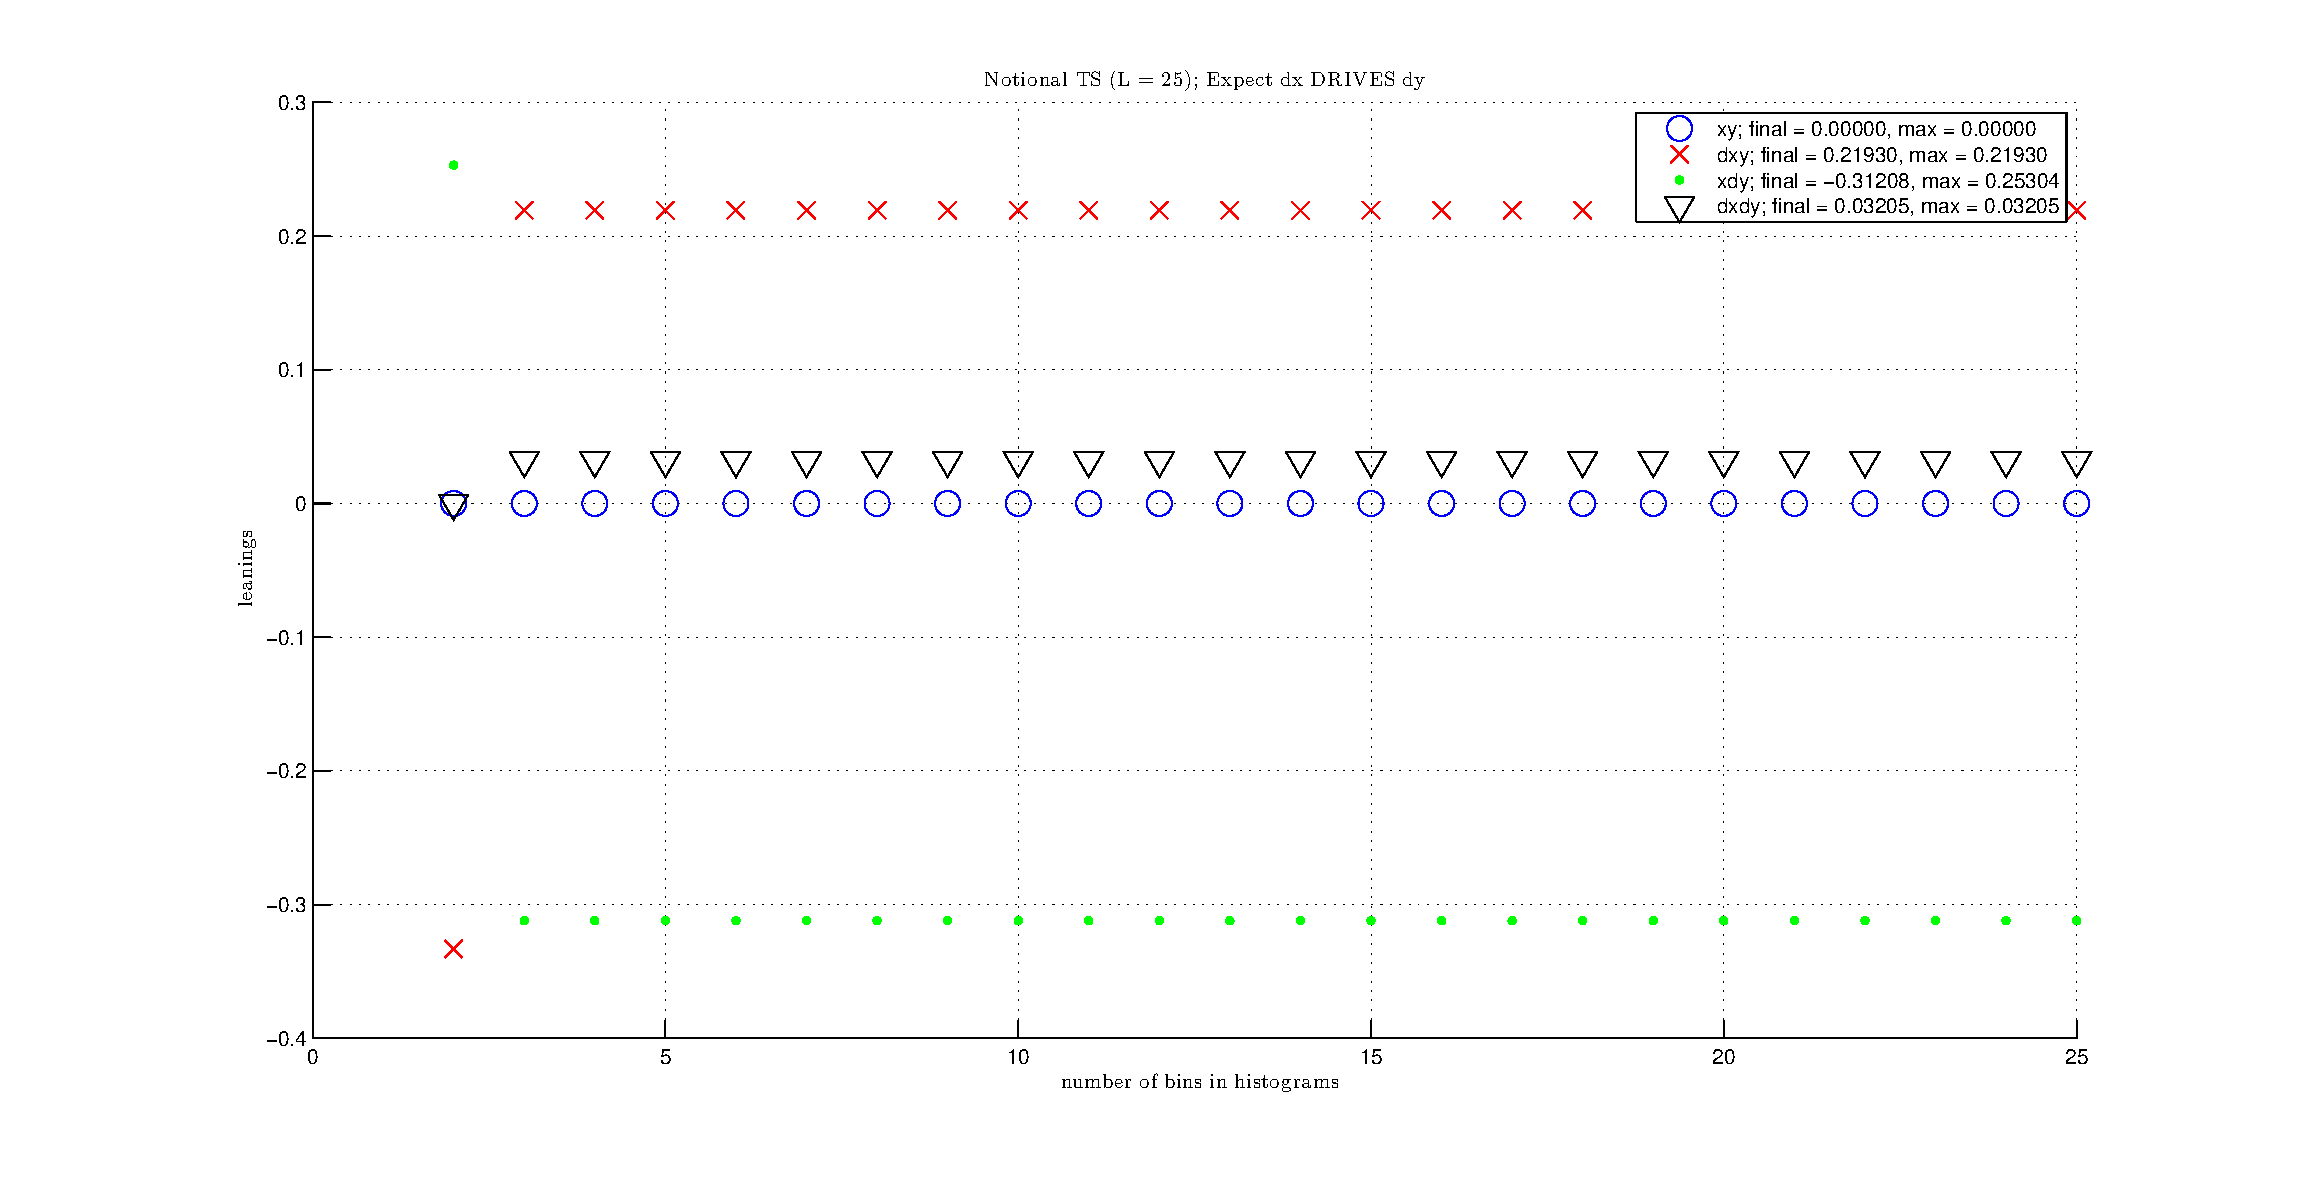
\includegraphics[scale=0.55]{notionalTS.eps}
%\end{figure}

This figure implies
$$
\begin{array}{ccc}
x & & y\\
\uparrow &\mathrel{\ooalign{\hss$\nearrow$\hss\cr$\nwarrow$}} & \uparrow\\
dx &\rightarrow & dy
\end{array}
$$
Consider the sine time series with varying noise levels and histogram bins:
%\begin{figure}[!H]
%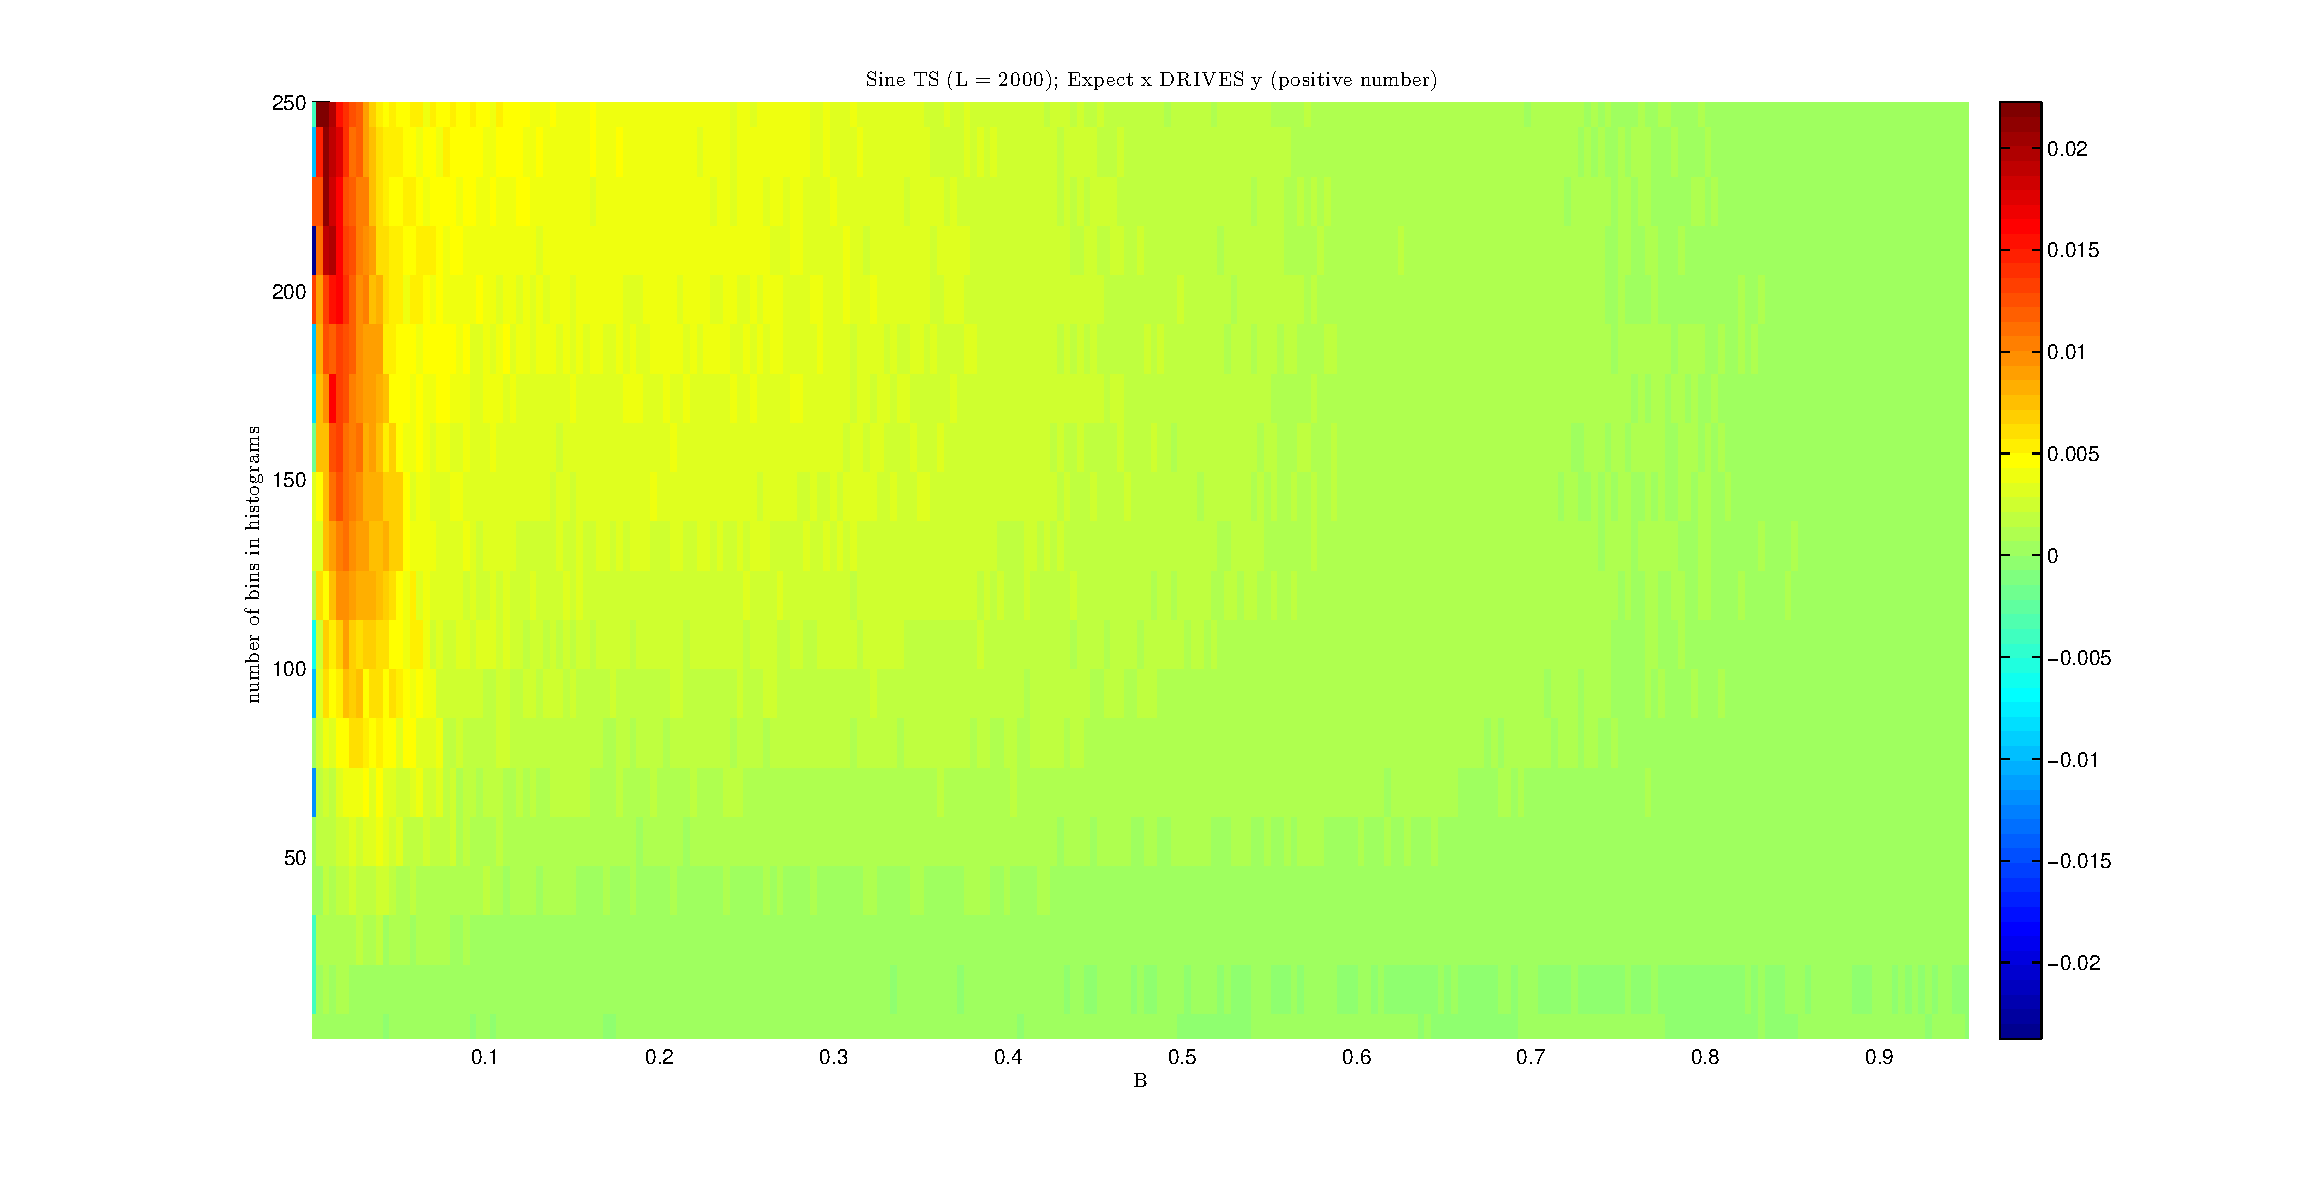
\includegraphics[scale=0.55]{SineTSxy.eps}
%\caption{Should be $X\rightarrow Y$; i.e.\ positive leaning (positive on colorbar)}
%\end{figure}
%\begin{figure}[!H]
%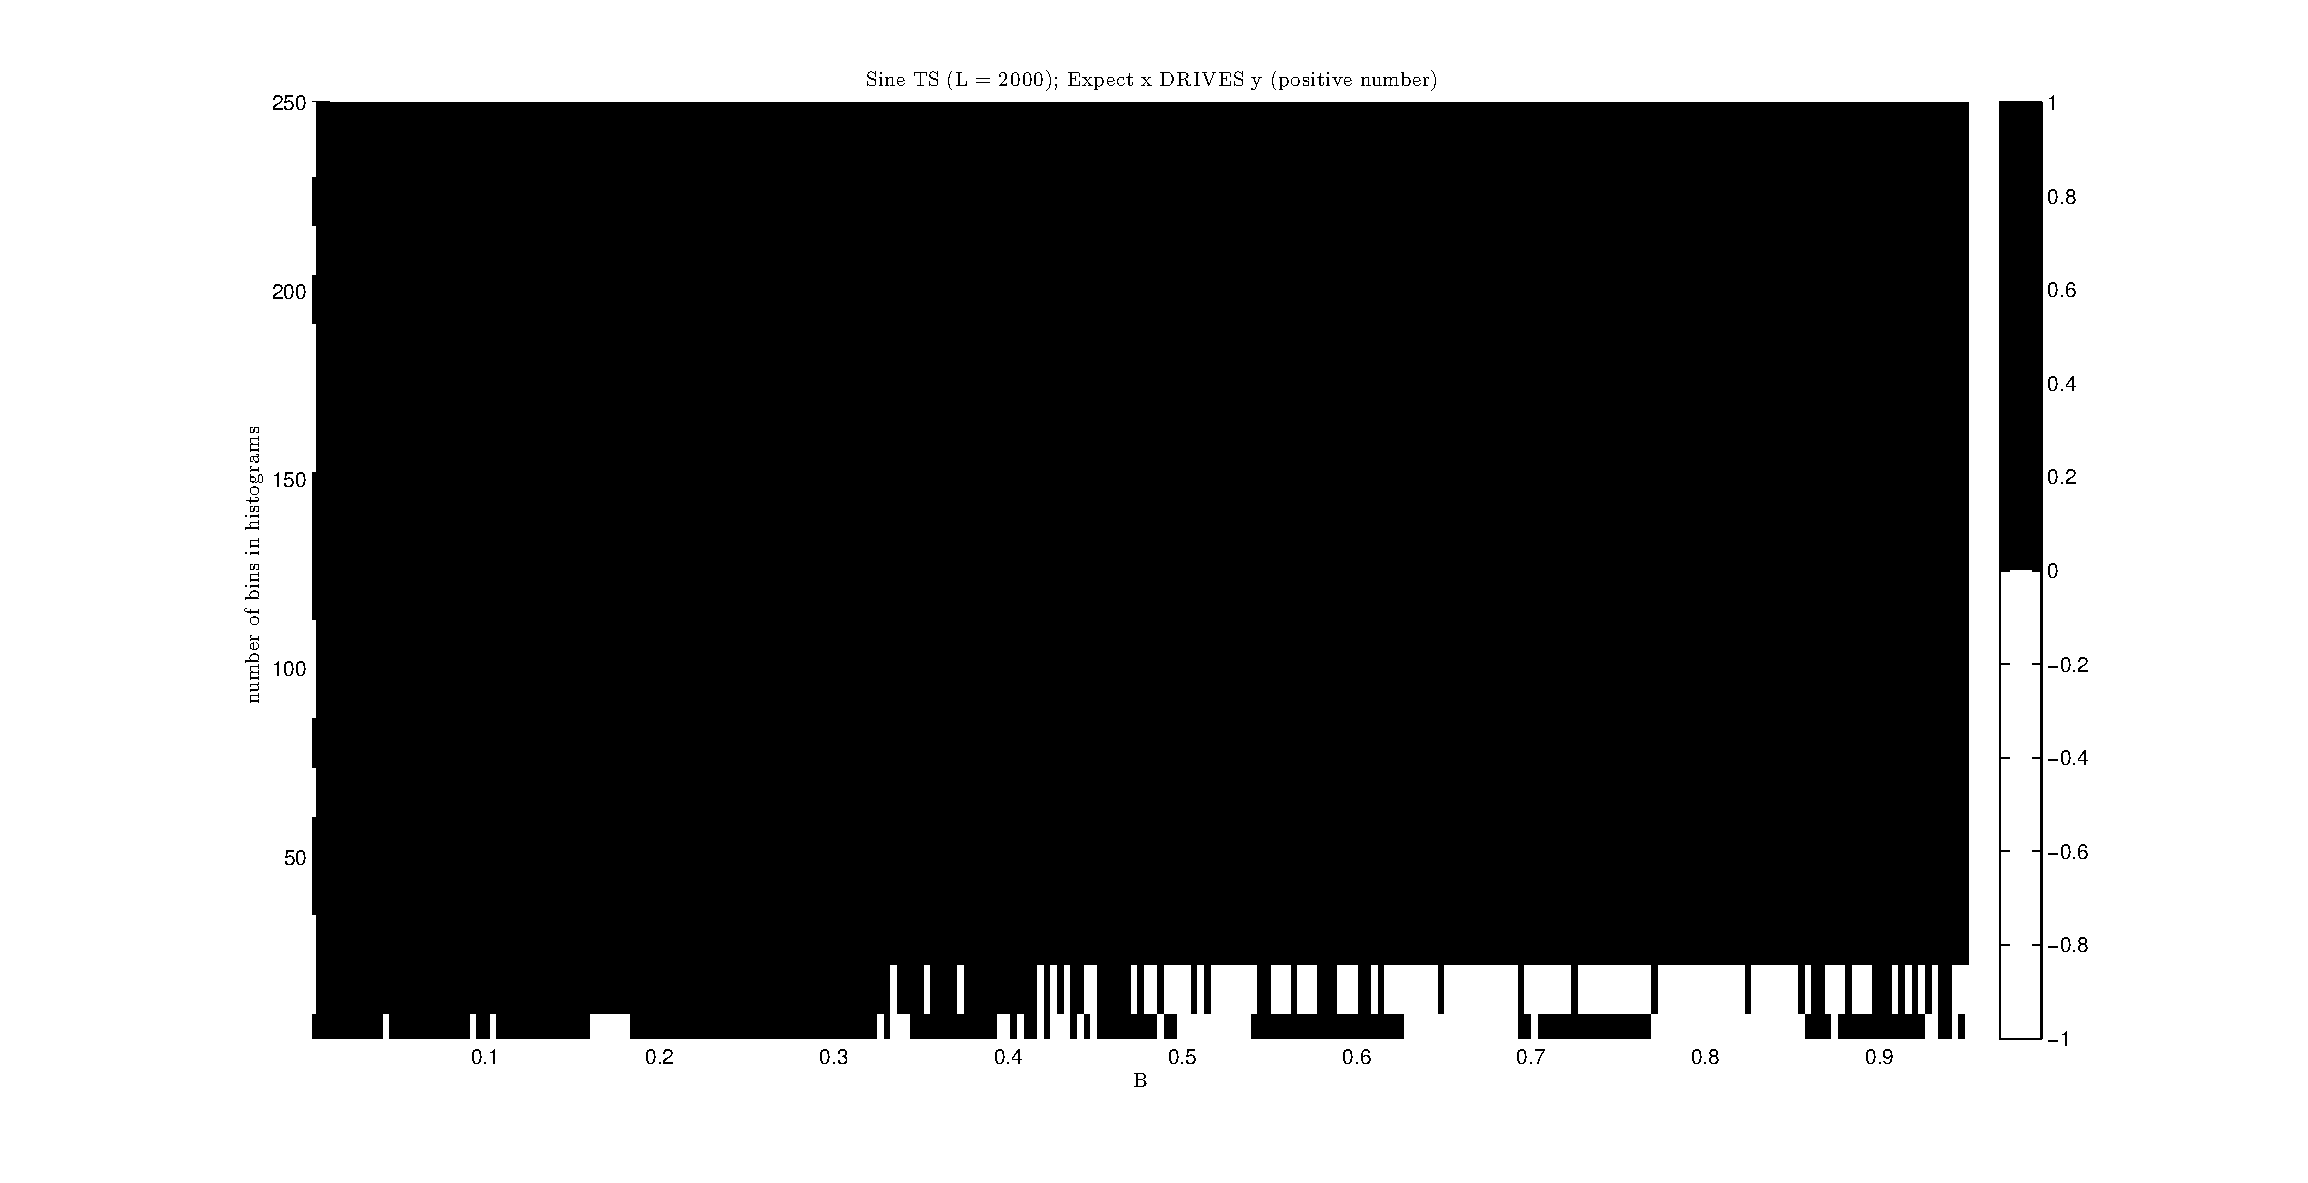
\includegraphics[scale=0.55]{SineTSxy_3C.eps}
%\caption{Should be $X\rightarrow Y$; i.e.\ positive leaning (positive on colorbar)}
%\end{figure}
%\begin{figure}[!H]
%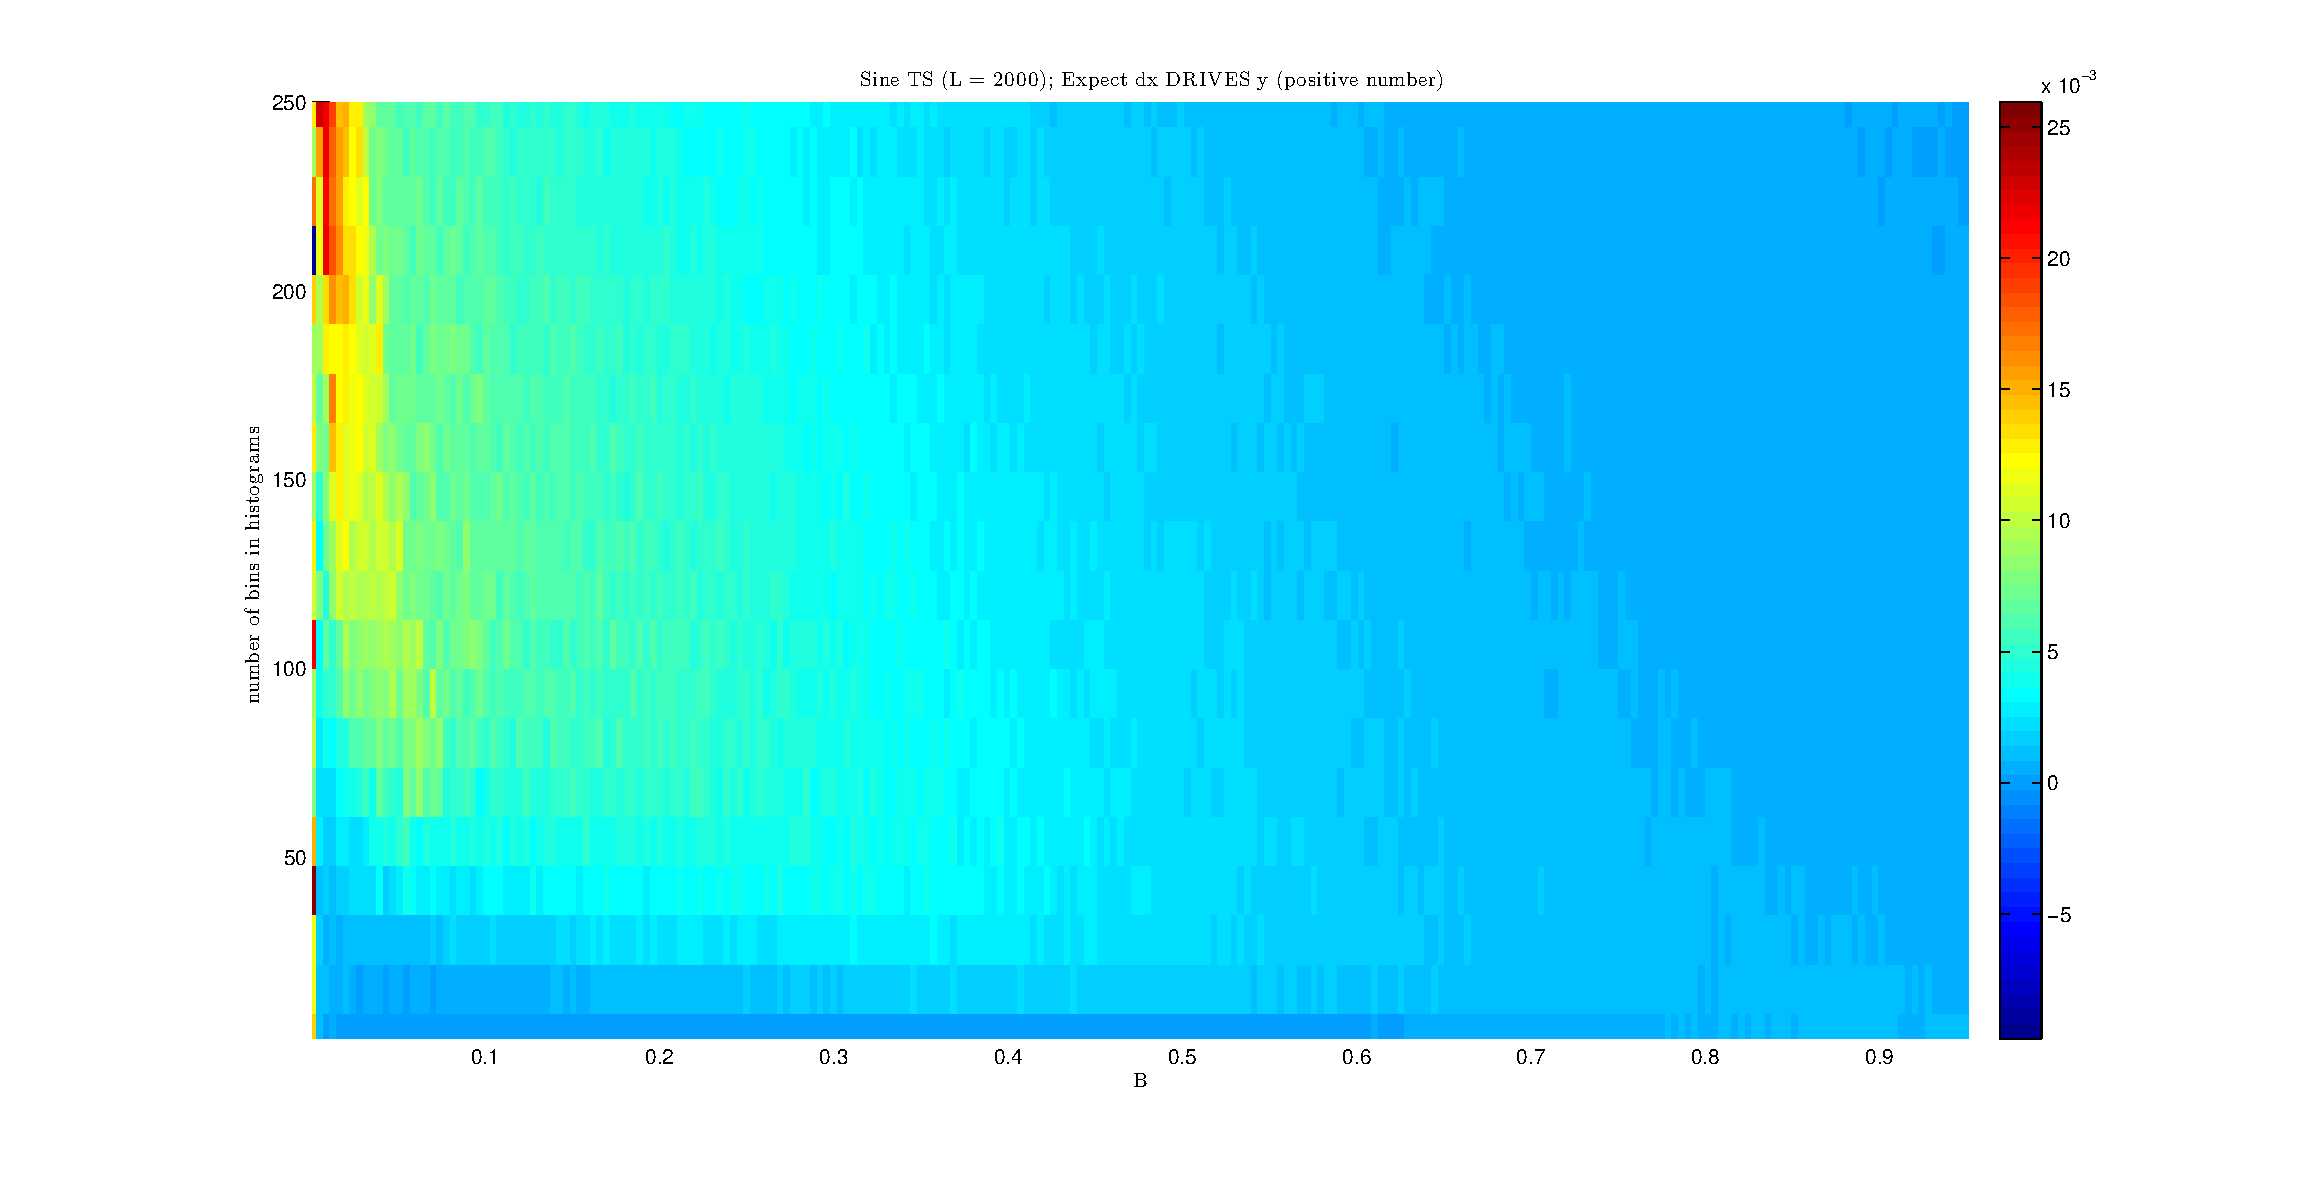
\includegraphics[scale=0.55]{SineTSdxy.eps}
%\caption{Should be $dX\rightarrow Y$; i.e.\ positive leaning (positive on colorbar)}
%\end{figure}
%\begin{figure}[!H]
%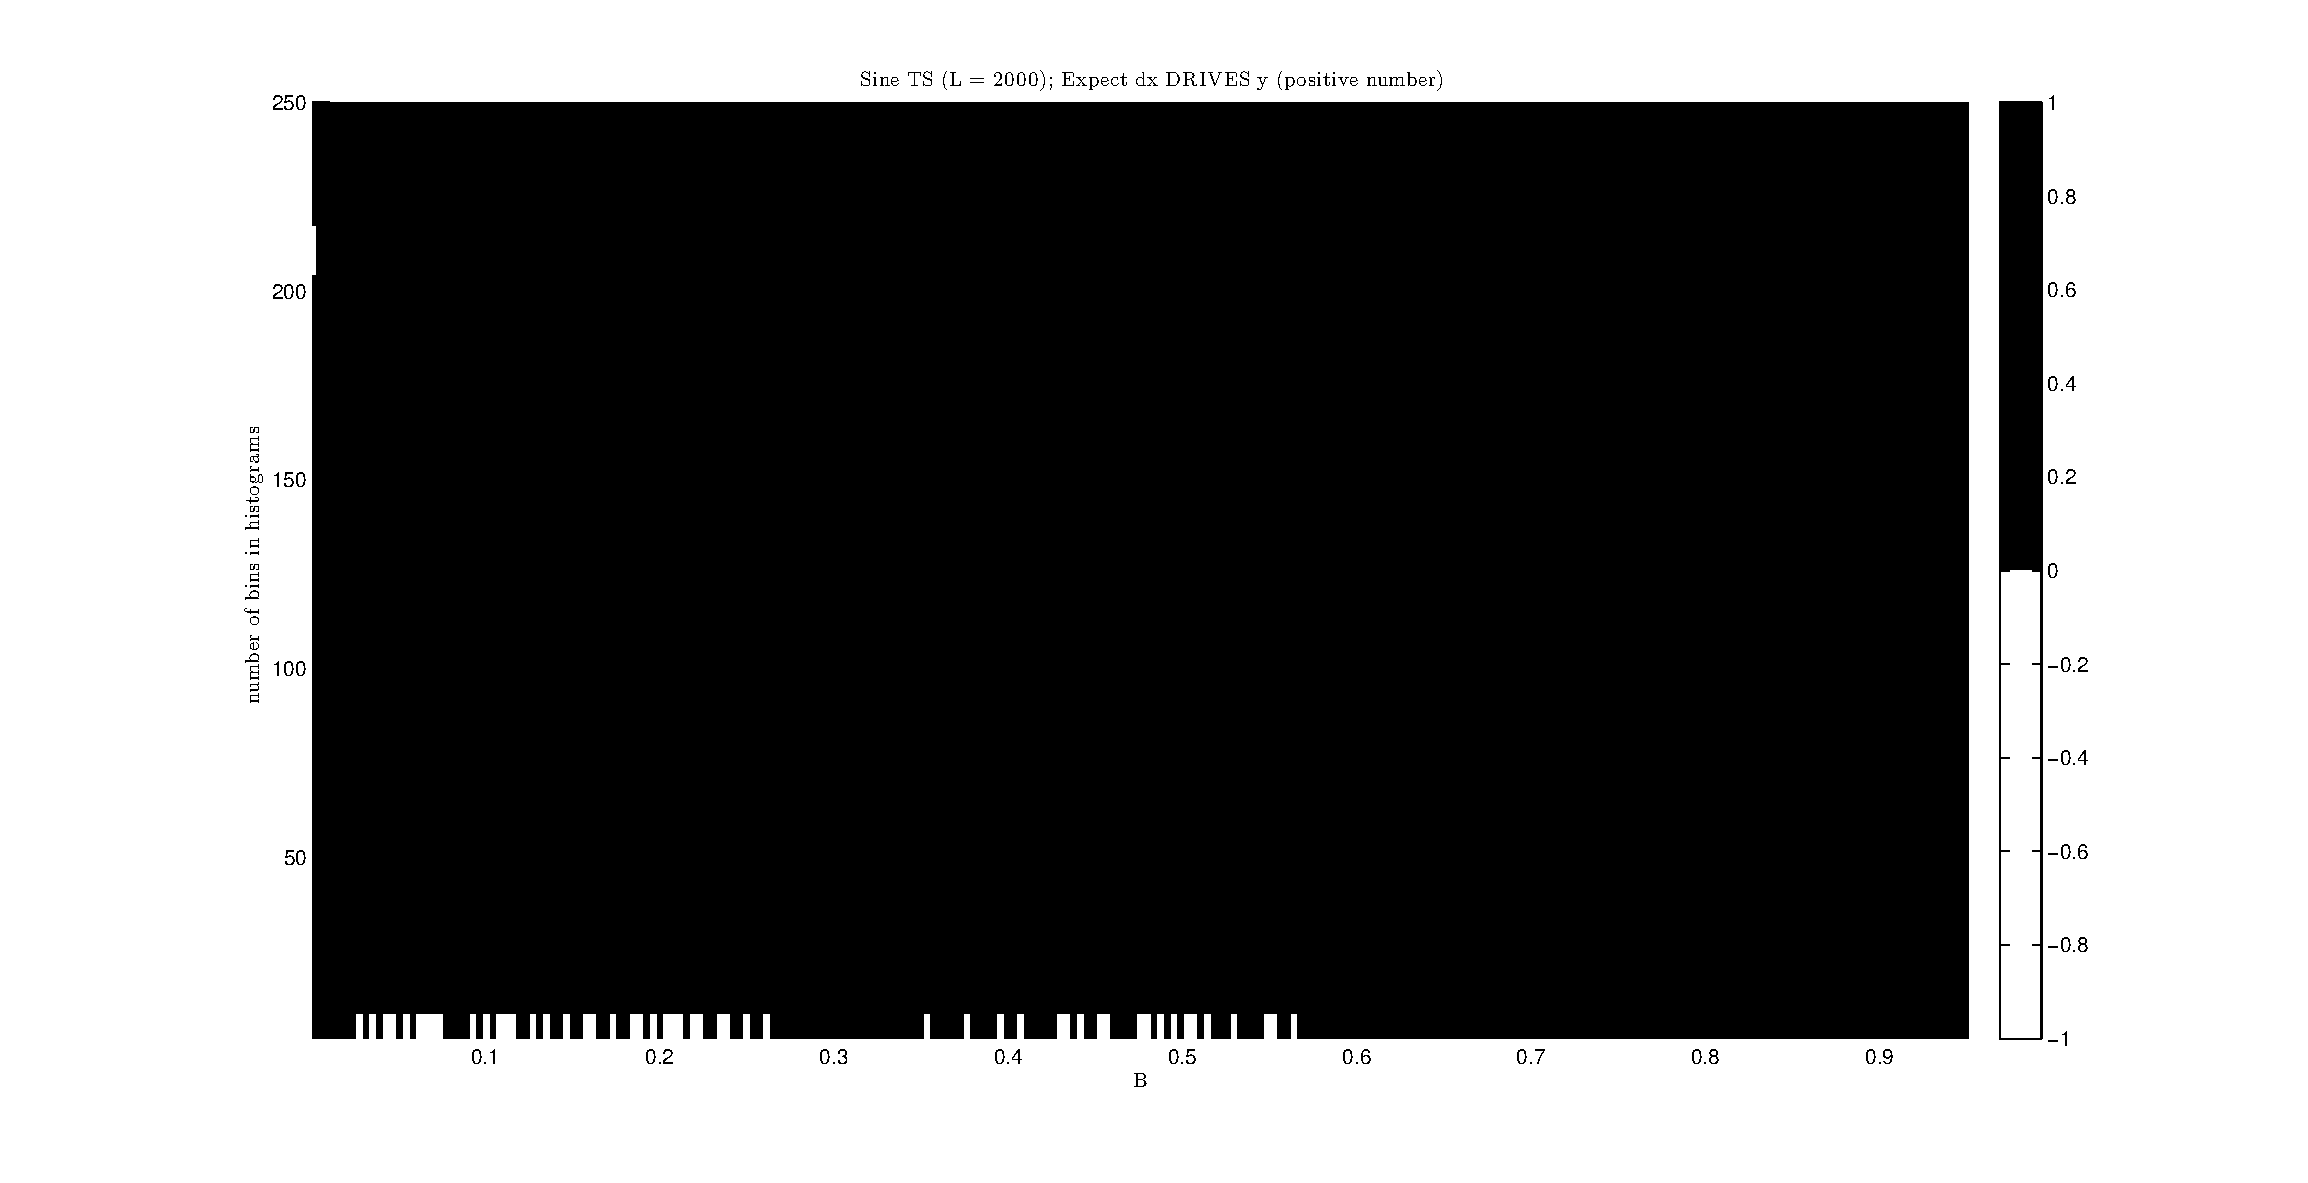
\includegraphics[scale=0.55]{SineTSdxy_3C.eps}
%\caption{Should be $dX\rightarrow Y$; i.e.\ positive leaning (positive on colorbar)}
%\end{figure}
%\begin{figure}[!H]
%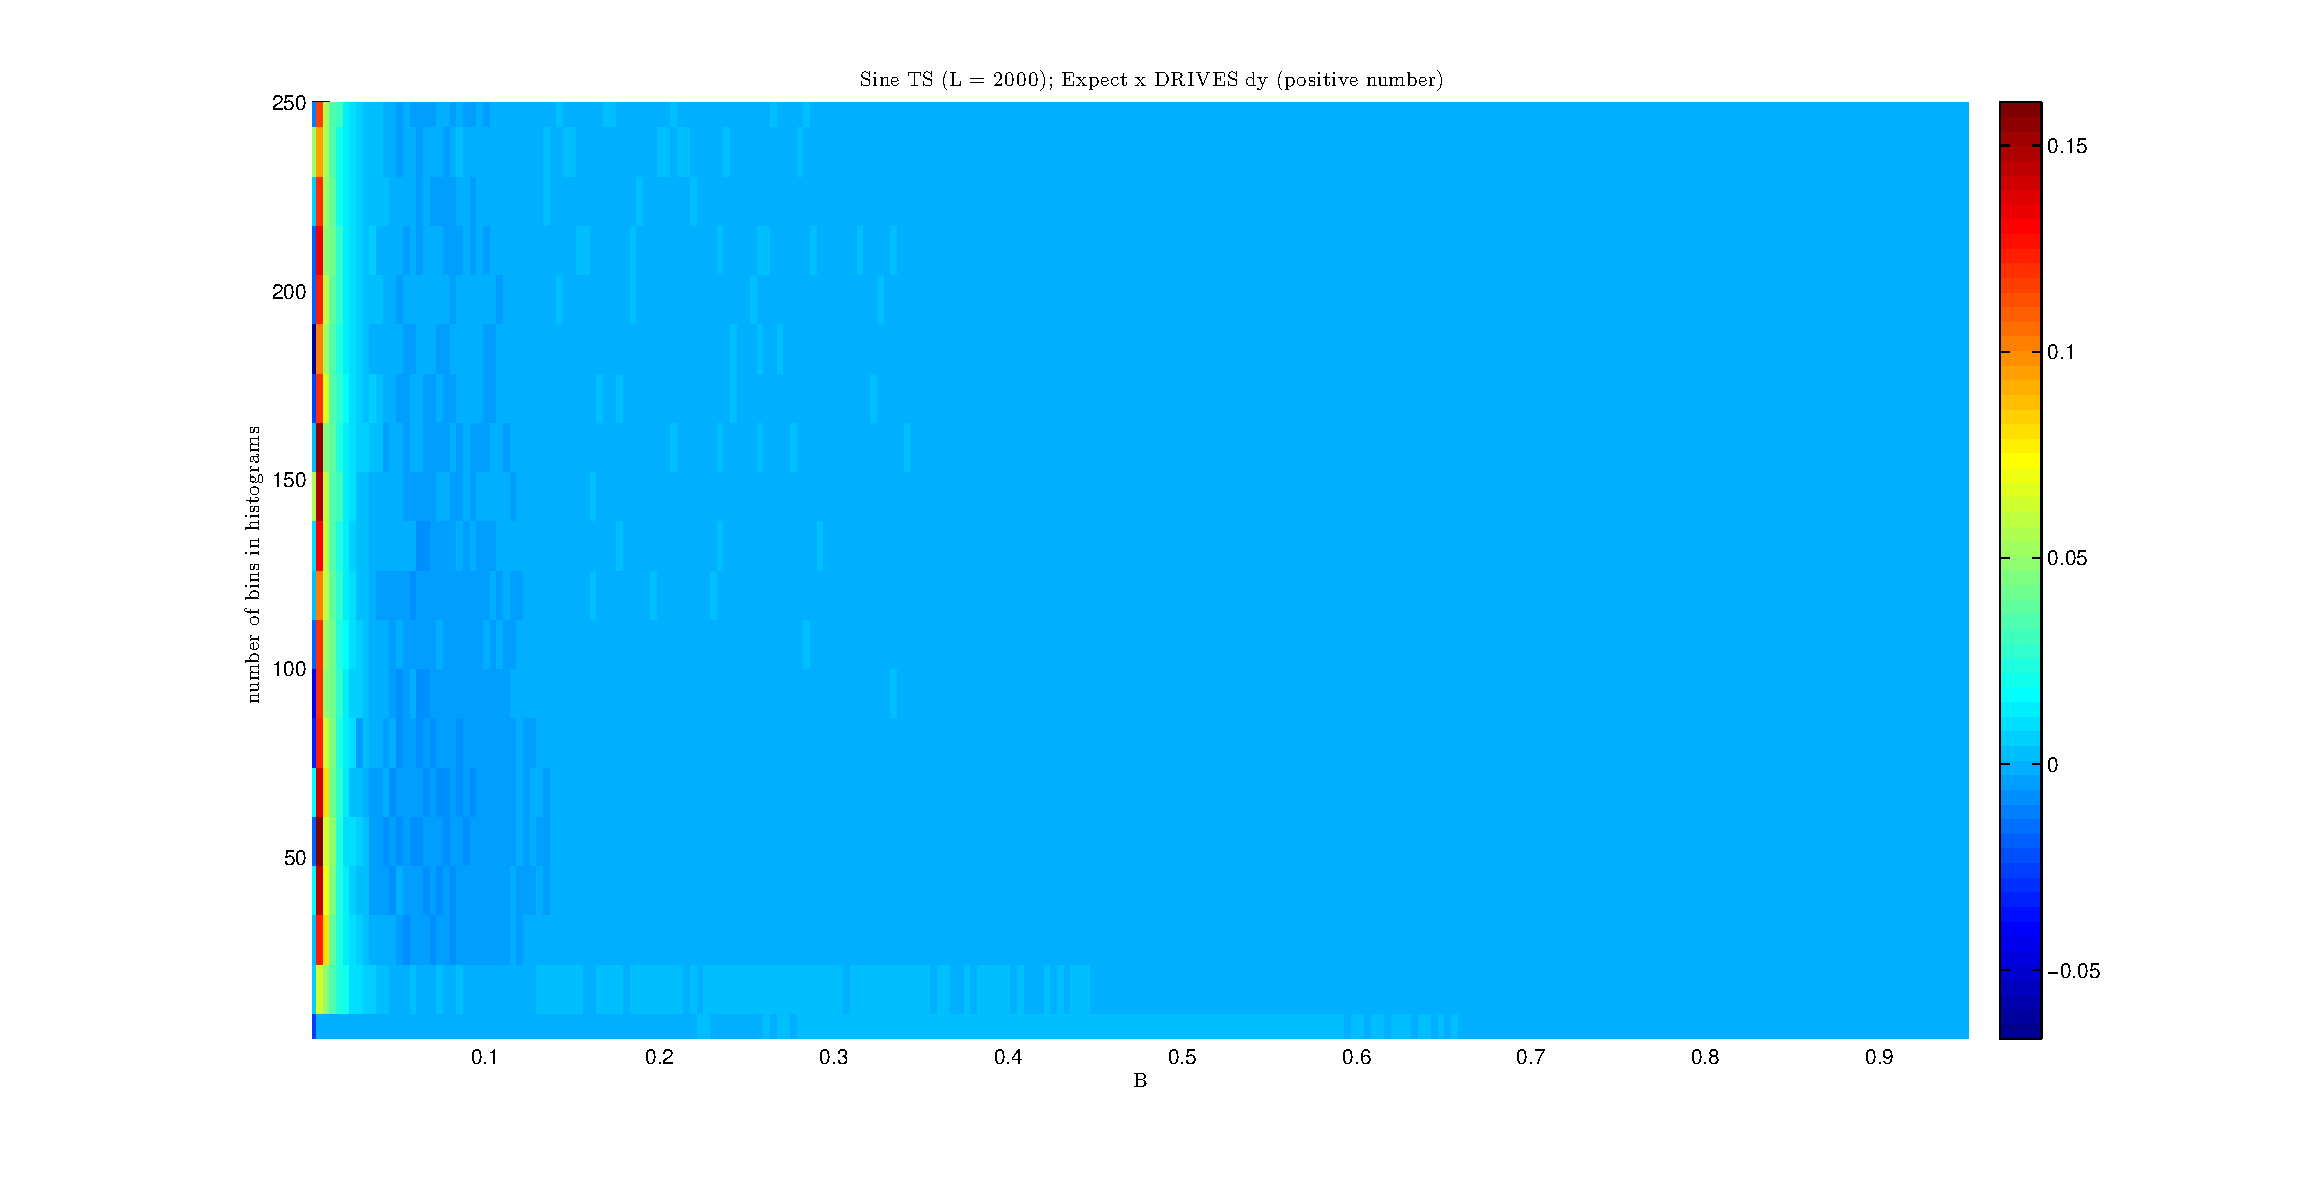
\includegraphics[scale=0.55]{SineTSxdy.eps}
%\caption{Should be $X\rightarrow dY$; i.e.\ positive leaning (positive on colorbar)}
%\end{figure}
%\begin{figure}[!H]
%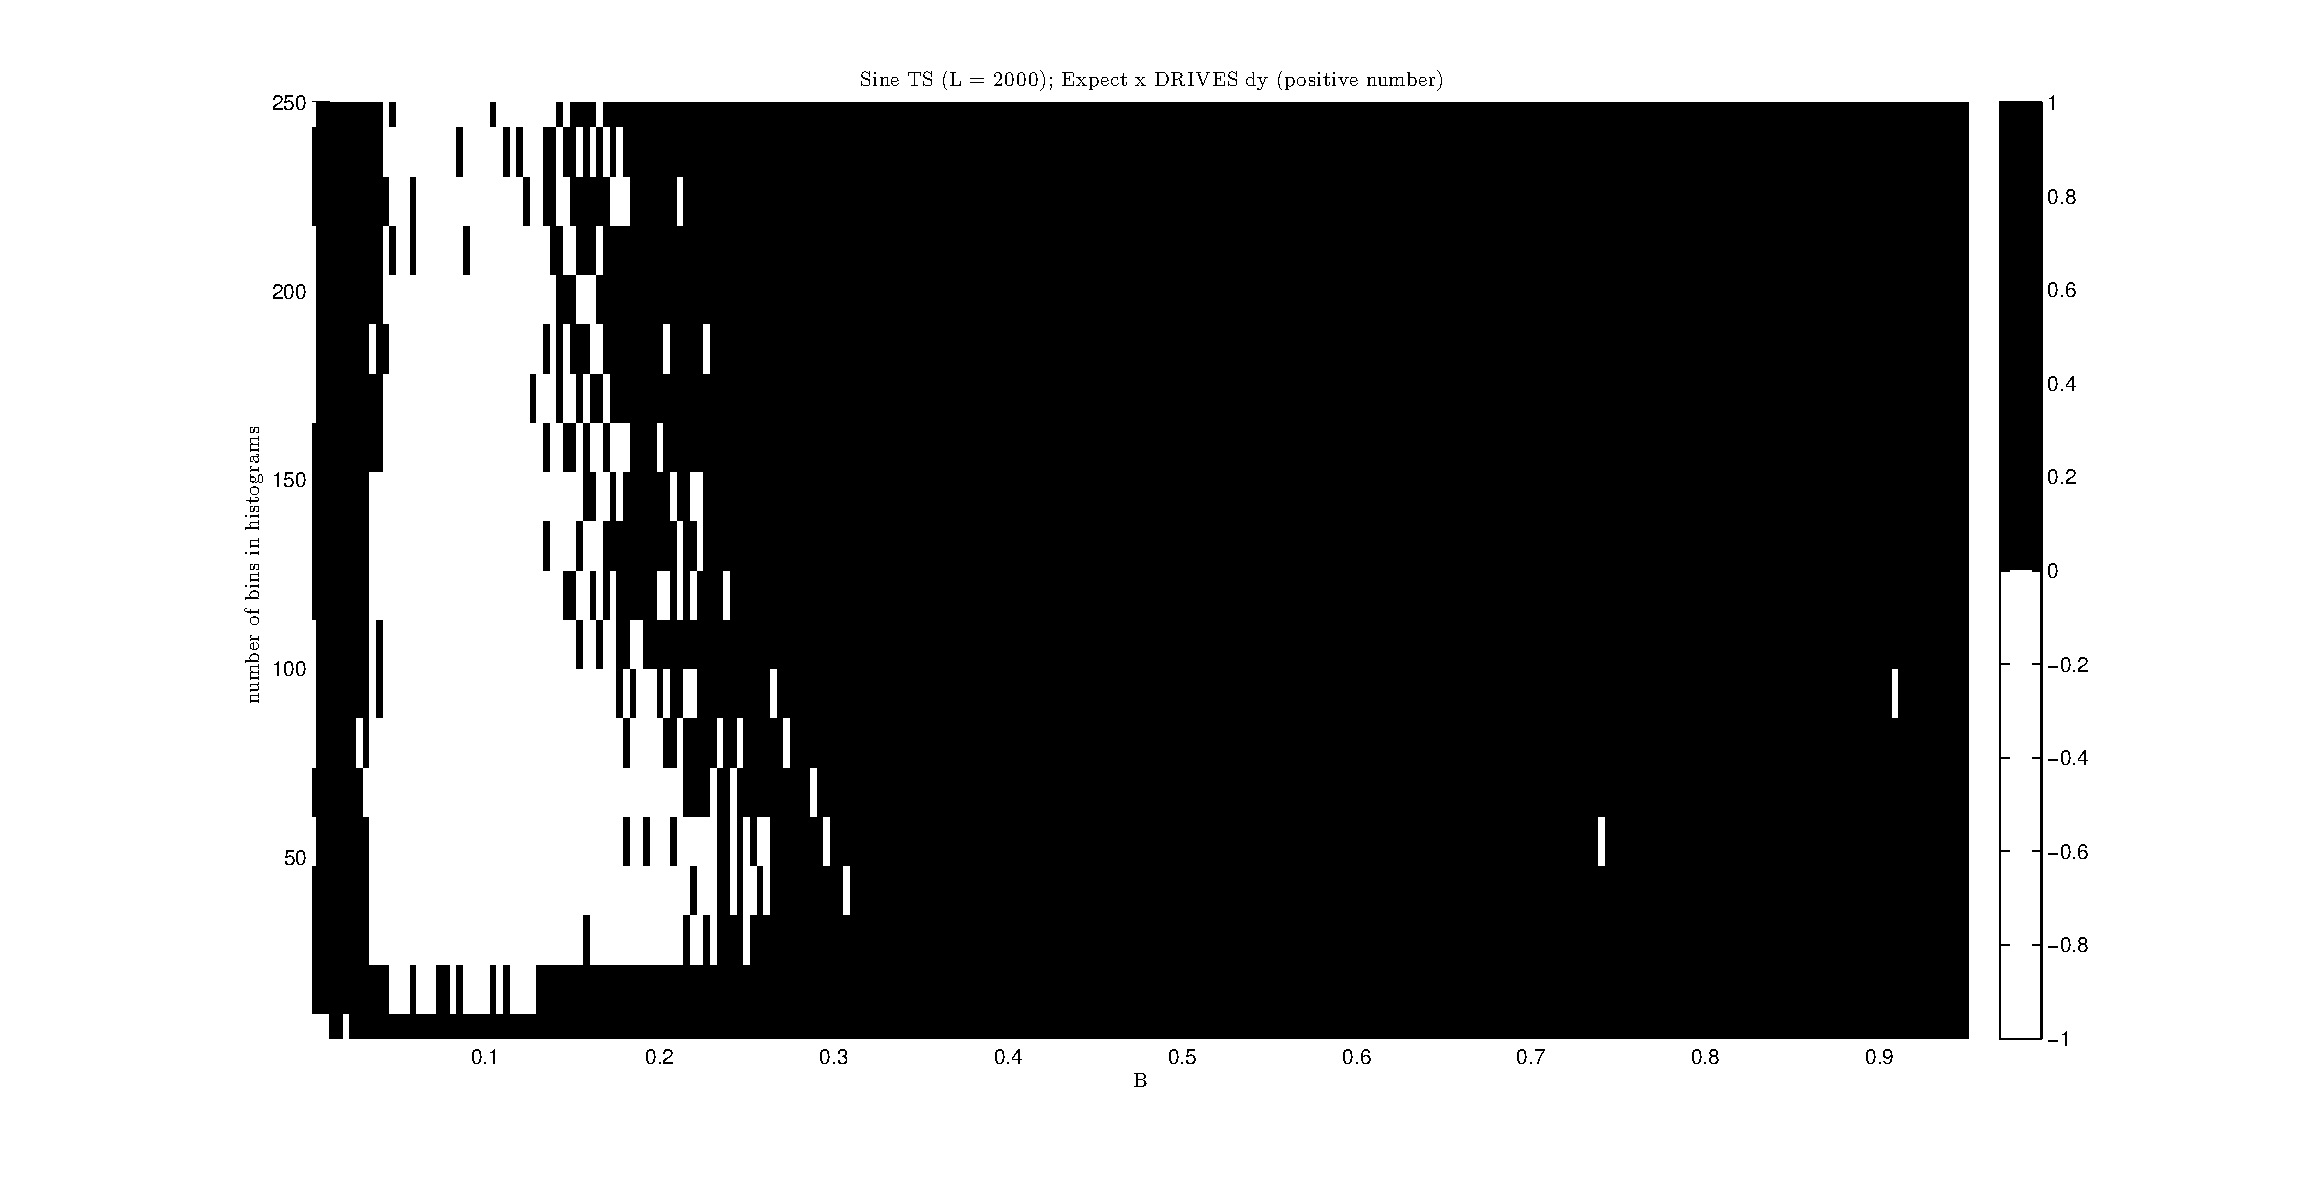
\includegraphics[scale=0.55]{SineTSxdy_3C.eps}
%\caption{Should be $X\rightarrow dY$; i.e.\ positive leaning (positive on colorbar)}
%\end{figure}
%\begin{figure}[!H]
%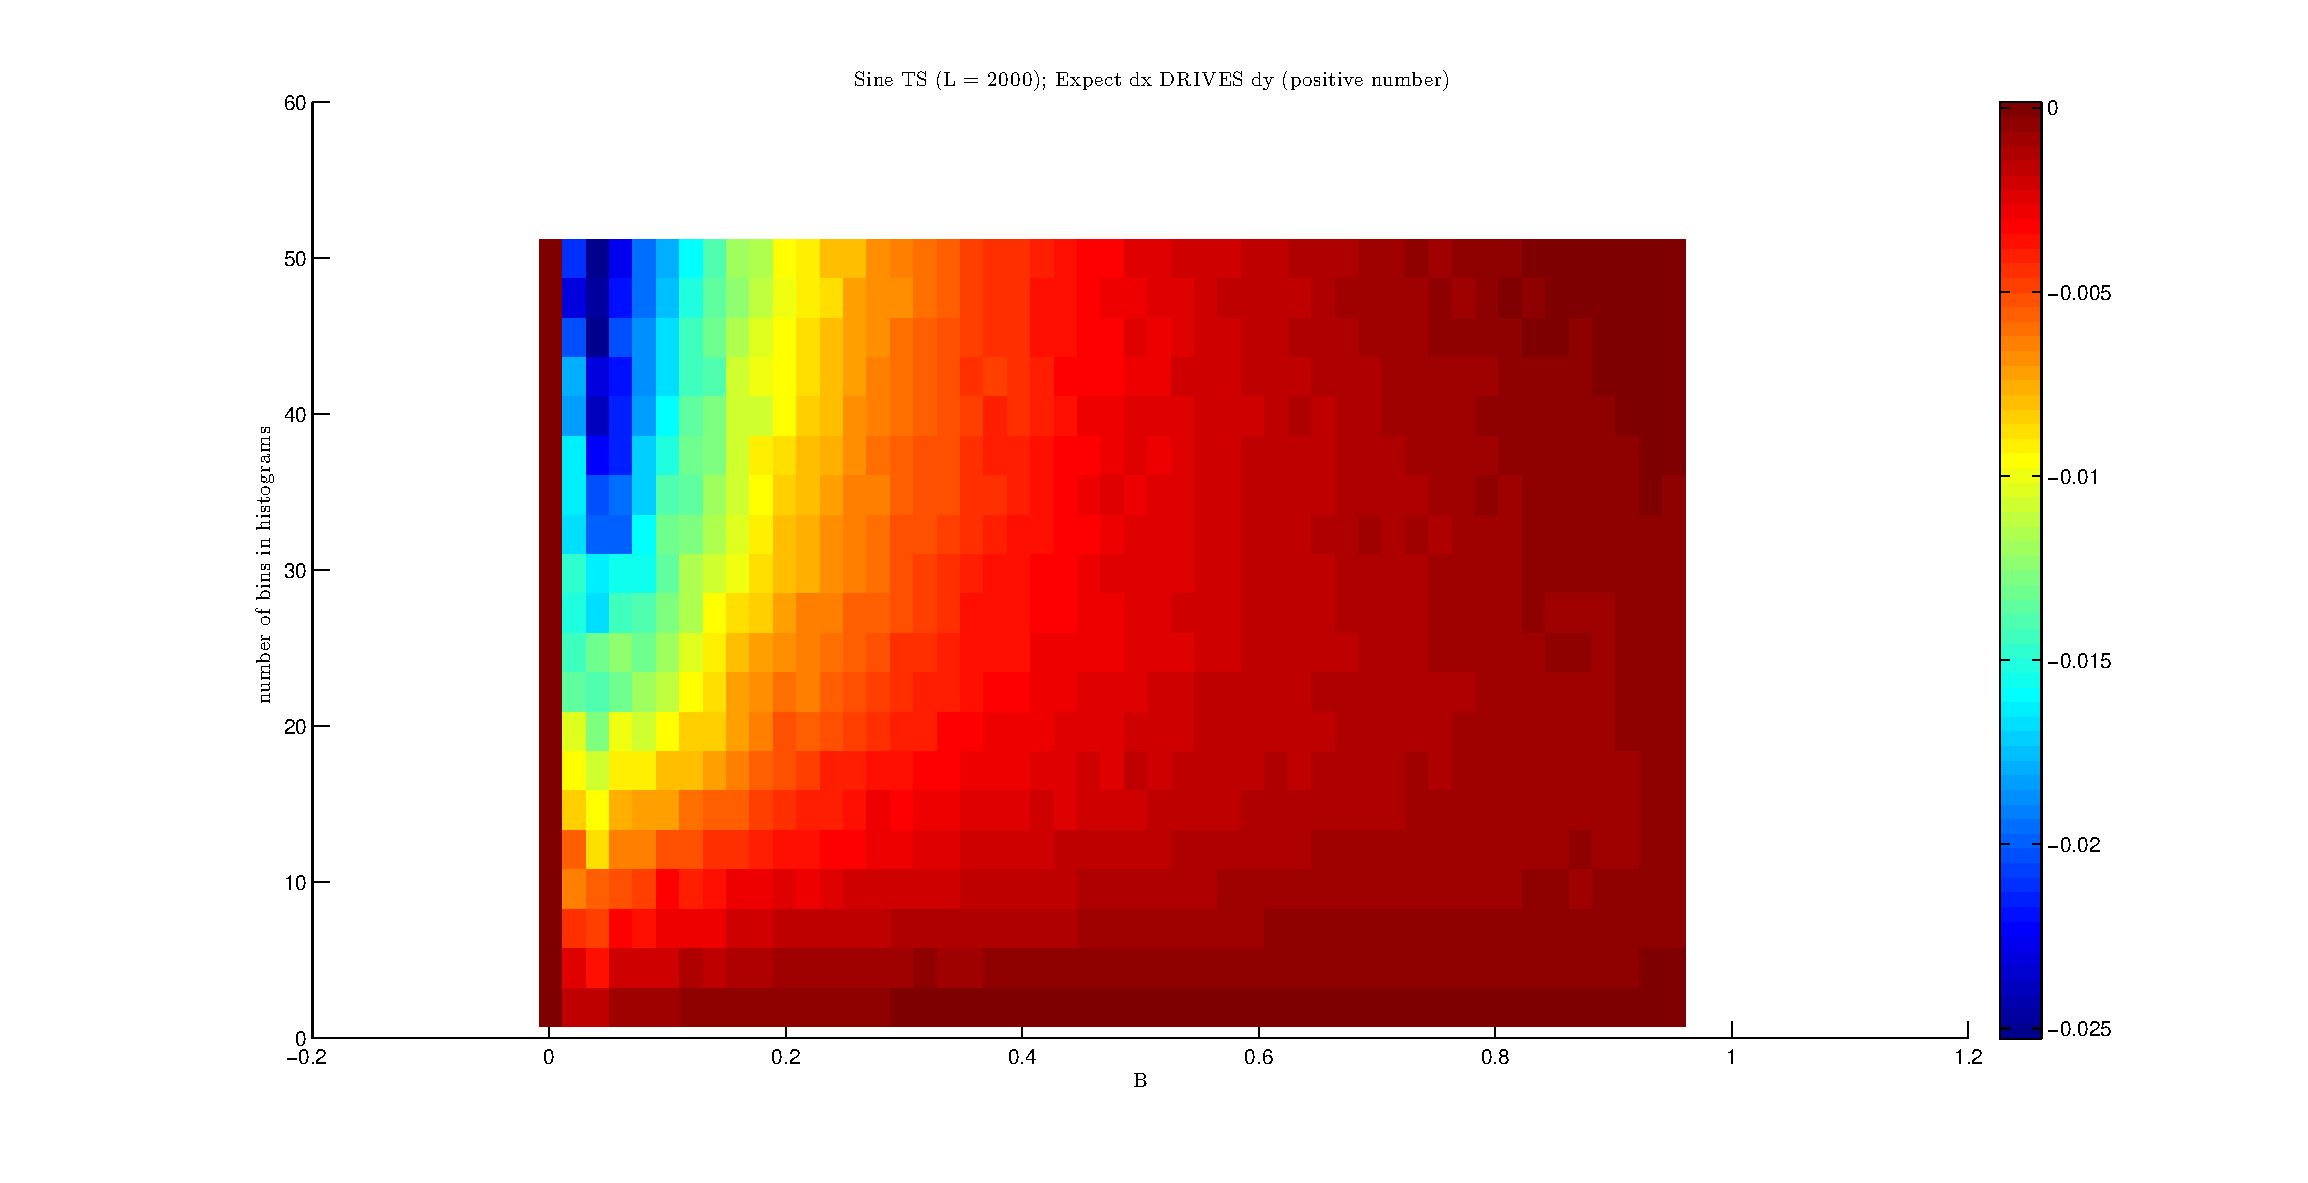
\includegraphics[scale=0.55]{SineTSdxdy.eps}
%\caption{Should be $dX\rightarrow dY$; i.e.\ positive leaning (positive on colorbar)}
%\end{figure}
%\begin{figure}[!H]
%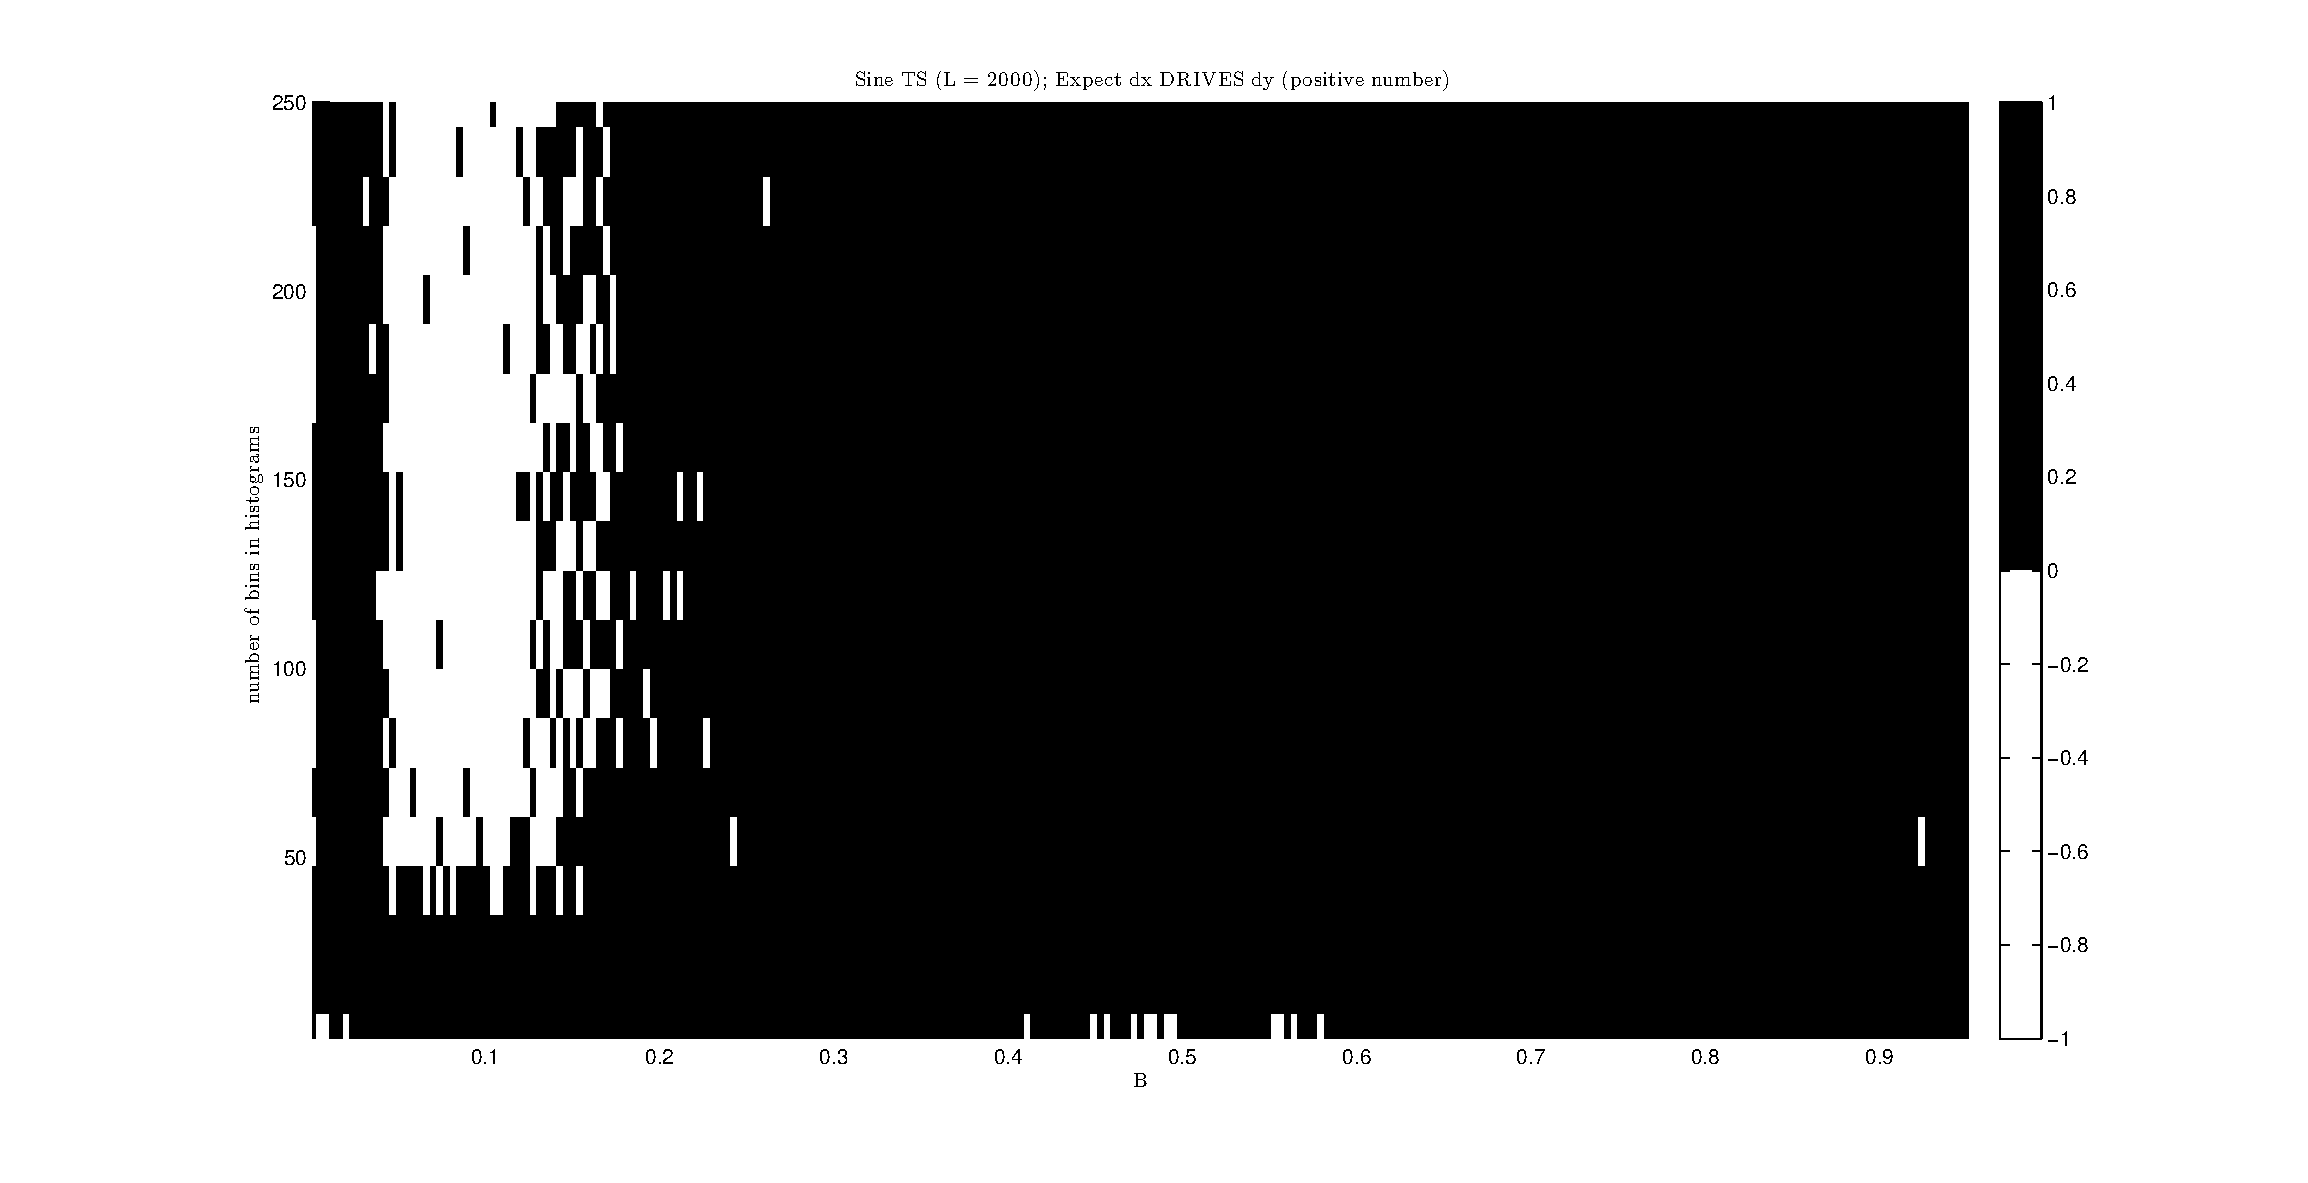
\includegraphics[scale=0.55]{SineTSdxdy_3C.eps}
%\caption{Should be $dX\rightarrow dY$; i.e.\ positive leaning (positive on colorbar)}
%\end{figure}

\newpage
\section{Example Time Series 1: Clean Impulse w/ Noisy Response}
Consider the time series $X\equiv\{x_t\}$ and $Y\equiv\{y_t=x_{t-1}+B\eta_t\}$ with $\eta_t\sim \mathcal{N}(0,1)$, $B\in[0,1]$, and $x_t = \kappa\;\forall t\in\mathbb{T}$ and $x_t = 0\;\forall t\notin\mathbb{T}$.  The $X$ peak value $\kappa$ and the set of times at which the peak values occur, $\mathbb{T}$, are assumed to not affect the causal inference between $X$ and $Y$ (assuming reasonable $\mathbb{T}$, e.g., assuming $\exists\;t\notin\mathbb{T}$).  The truth for this example time series is $X\rightarrow Y$.

The following set of ``leaning reports'' were generated a library length $L=20$, $B=0.3$, $\mathbb{T} = \{1,5,15\}$, and $\kappa = 2$; the full command was 
\begin{verbatim}
[x,y] = wTS(20,0.3,[1 5 15],[2 2 2]);
\end{verbatim}
The leaning reports differ only in the number of bins used in the leaning calculations.  The report commands are shown for clarity.

\begin{verbatim}
>> leaning_report(x,y,3,1e-6,[-2,-1,0,1,2])
-------------------------
Lagged Leanings:
  [lag,leaning] :: guess
  -2,0.2150162 :: x_{t+-2}->y
  -1,0.2649977 :: x_{t+-1}->y
  0,0.3138691 :: x_{t+0}->y
  1,0.1623932 :: x_{t+1}->y
  2,0.1846154 :: x_{t+2}->y
-------------------------
LIR Leanings:
  [ID,leaning] :: guess
  (x,y),0.3138691 :: x->y
  (dx,y),-0.2027365 :: y->dx
  (dx,dy),0.0150518 :: dx->dy
  (x,dy),0.4682899 :: x->dy
  (dx,x),-0.6050109 :: x->dx
  (dy,y),-0.1274689 :: y->dy
  (x&dx,y),-0.0168633 :: y->x&dx
  (y&dy,x),-0.2476780 :: x->y&dy
  (x&dx,y&dy),0.0034400 :: x&dx->y&dy
\end{verbatim} 
\begin{verbatim}
>> leaning_report(x,y,5,1e-6,[-2,-1,0,1,2])
-------------------------
Lagged Leanings:
  [lag,leaning] :: guess
  -2,0.6428571 :: x_{t+-2}->y
  -1,0.6269024 :: x_{t+-1}->y
  0,0.6431373 :: x_{t+0}->y
  1,0.5428571 :: x_{t+1}->y
  2,0.5743590 :: x_{t+2}->y
-------------------------
LIR Leanings:
  [ID,leaning] :: guess
  (x,y),0.6431373 :: x->y
  (dx,y),0.0603486 :: dx->y
  (dx,dy),-0.0329019 :: dy->dx
  (x,dy),0.2580981 :: x->dy
  (dx,x),-0.6050109 :: x->dx
  (dy,y),-0.0016151 :: y->dy
  (x&dx,y),-0.1065015 :: y->x&dx
  (y&dy,x),-0.1981424 :: x->y&dy
  (x&dx,y&dy),0.0995528 :: x&dx->y&dy
\end{verbatim} 
\begin{verbatim}
>> leaning_report(x,y,10,1e-6,[-2,-1,0,1,2])
-------------------------
Lagged Leanings:
  [lag,leaning] :: guess
  -2,0.4158482 :: x_{t+-2}->y
  -1,0.3853554 :: x_{t+-1}->y
  0,0.3980392 :: x_{t+0}->y
  1,0.3204365 :: x_{t+1}->y
  2,0.3225962 :: x_{t+2}->y
-------------------------
LIR Leanings:
  [ID,leaning] :: guess
  (x,y),0.3980392 :: x->y
  (dx,y),0.0008913 :: dx->y
  (dx,dy),-0.0010890 :: dy->dx
  (x,dy),0.1571900 :: x->dy
  (dx,x),-0.6050109 :: x->dx
  (dy,y),-0.0325069 :: y->dy
  (x&dx,y),-0.0548762 :: y->x&dx
  (y&dy,x),-0.2935443 :: x->y&dy
  (x&dx,y&dy),0.0510836 :: x&dx->y&dy
\end{verbatim} 
\begin{verbatim}
>> leaning_report(x,y,15,1e-6,[-2,-1,0,1,2])
-------------------------
Lagged Leanings:
  [lag,leaning] :: guess
  -2,0.3407955 :: x_{t+-2}->y
  -1,0.3331653 :: x_{t+-1}->y
  0,0.3445715 :: x_{t+0}->y
  1,0.2874359 :: x_{t+1}->y
  2,0.2793407 :: x_{t+2}->y
-------------------------
LIR Leanings:
  [ID,leaning] :: guess
  (x,y),0.3445715 :: x->y
  (dx,y),0.0389137 :: dx->y
  (dx,dy),0.0063290 :: dx->dy
  (x,dy),0.1098856 :: x->dy
  (dx,x),-0.6050109 :: x->dx
  (dy,y),-0.0129562 :: y->dy
  (x&dx,y),-0.0652997 :: y->x&dx
  (y&dy,x),-0.3002158 :: x->y&dy
  (x&dx,y&dy),0.0510836 :: x&dx->y&dy
\end{verbatim}
Consider the lagged leaning
\begin{verbatim}
x_{t+-1}
\end{verbatim}
which is 
\begin{eqnarray}
\Delta_{y_t x_{t-1}} &=& \langle \rho_{y_t x_{t-1}}\rangle - \langle \rho_{x_{t-1} y_t}\rangle\\
&=& \langle P(y_t| x_{t-1}) - P(y_t| x_{t^\prime\neq t-1})\rangle - \langle P(x_{t-1} |y_t)-P(x_{t-1} |y_{t^\prime\neq t})\rangle
\end{eqnarray}
%\begin{figure}[!H]
%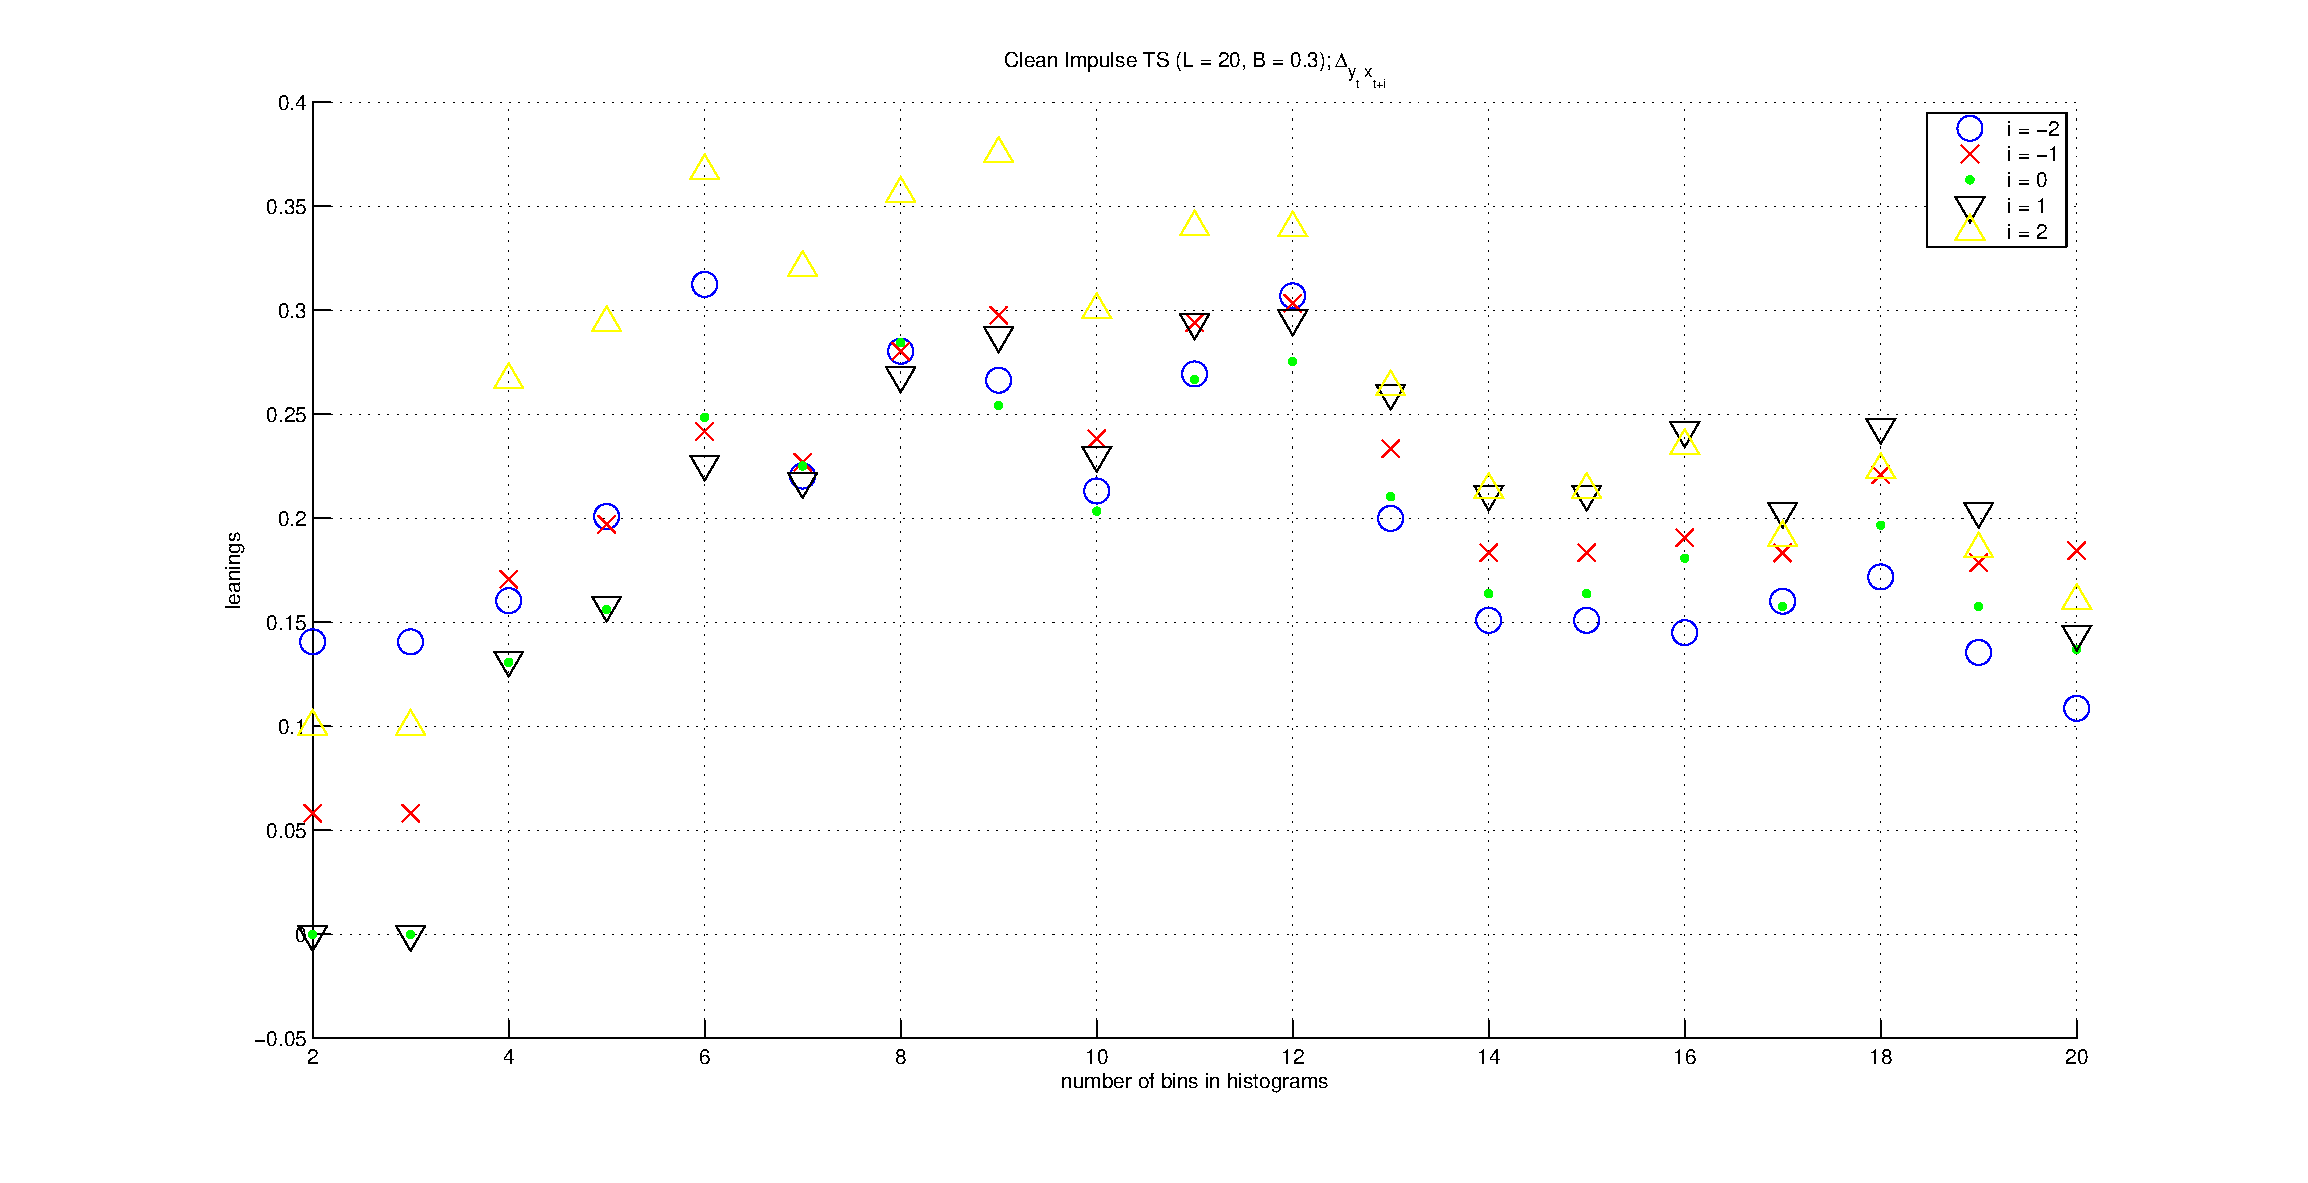
\includegraphics[scale=0.55]{laggedleans_wTS.eps}
%\caption{Should be $x\rightarrow y$; i.e.\ positive leaning}
%\end{figure}

\newpage
Consider 
\begin{verbatim}
[x,y] = wTS(20,0,[1 5 15],[2 2 2]);
\end{verbatim}
which is the clean impulse time series from above with no noise in the response, i.e.\ $B=0$.  The penchants $\rho_{yx}$, $\rho_{xy}$ and the leaning $\Delta_{yx}$ are all shown below.
\begin{figure}[!H]
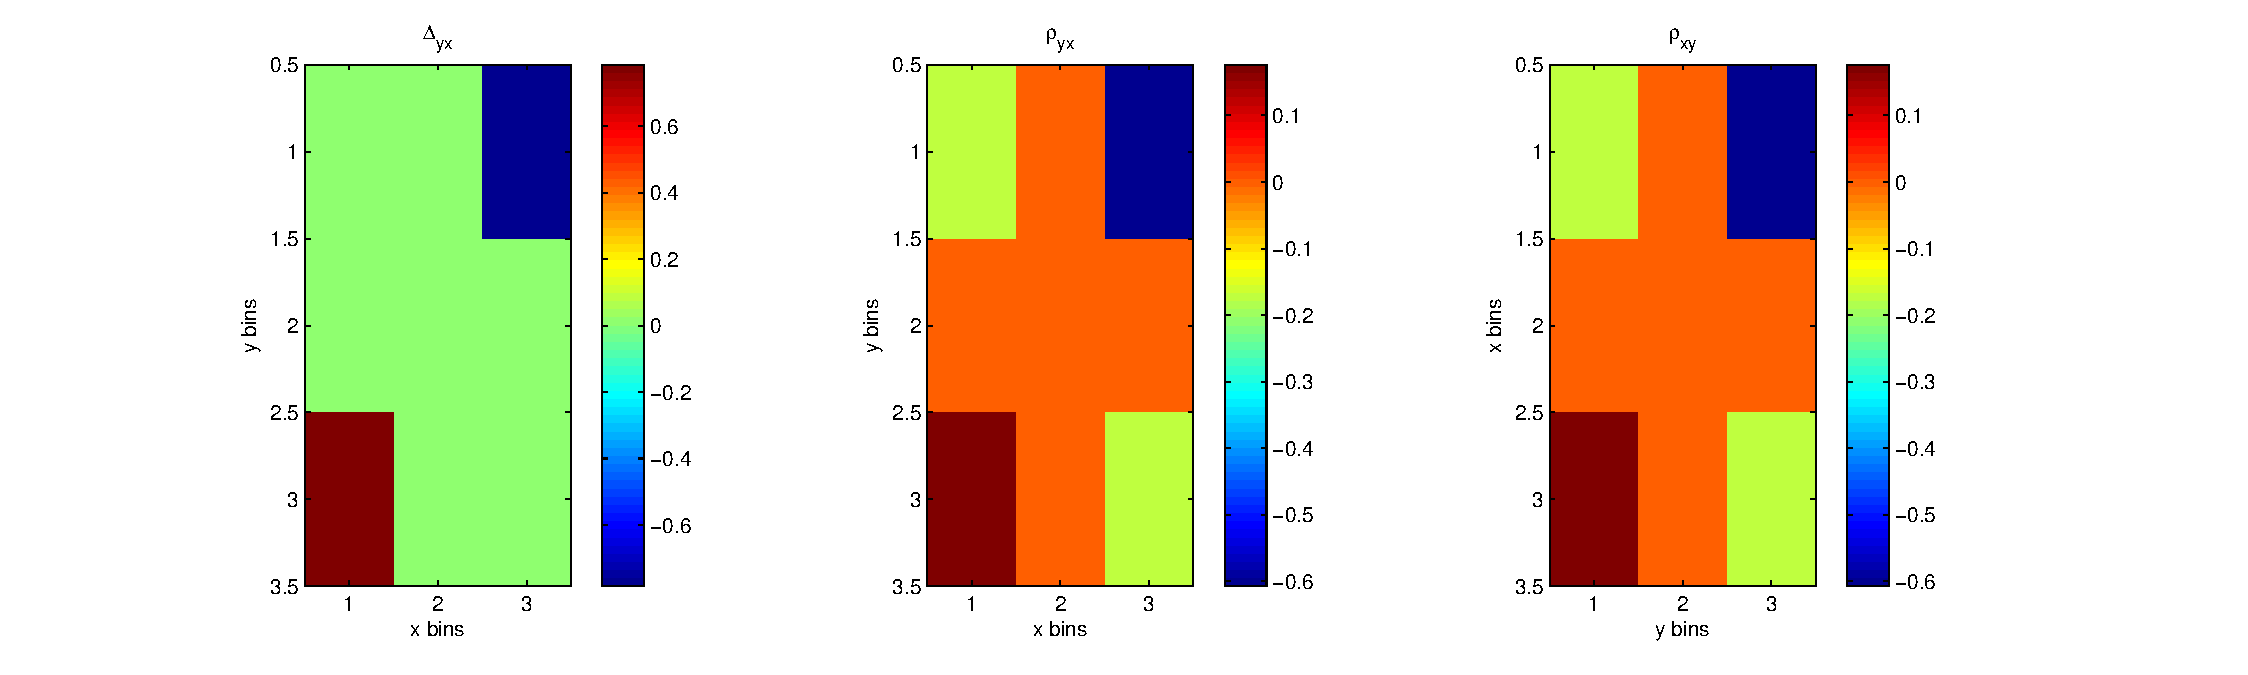
\includegraphics[scale=0.55]{sTWpenIMG.eps}
\end{figure}
$$
\rho_{yx} = \begin{array}{ccc}
   -0.1765    &     0  & -0.6078\\
         0    &     0  &      0\\
    0.1765    &     0  & -0.1765
\end{array}
$$
$$
\rho_{xy} = \begin{array}{ccc}
   -0.1765   &      0 &  -0.6078\\
         0   &      0 &        0\\
    0.1765   &      0 &  -0.1765
\end{array}
$$
$$
\Delta_{yx} = \begin{array}{ccc}
         0    &     0  & -0.7843\\
         0    &     0  &       0\\
    0.7843    &     0  &       0
\end{array}
$$

\begin{verbatim}
[x,y] = wTS(20,0,[1 5 15],[2 2 2]);
\end{verbatim}
\begin{figure}[!H]
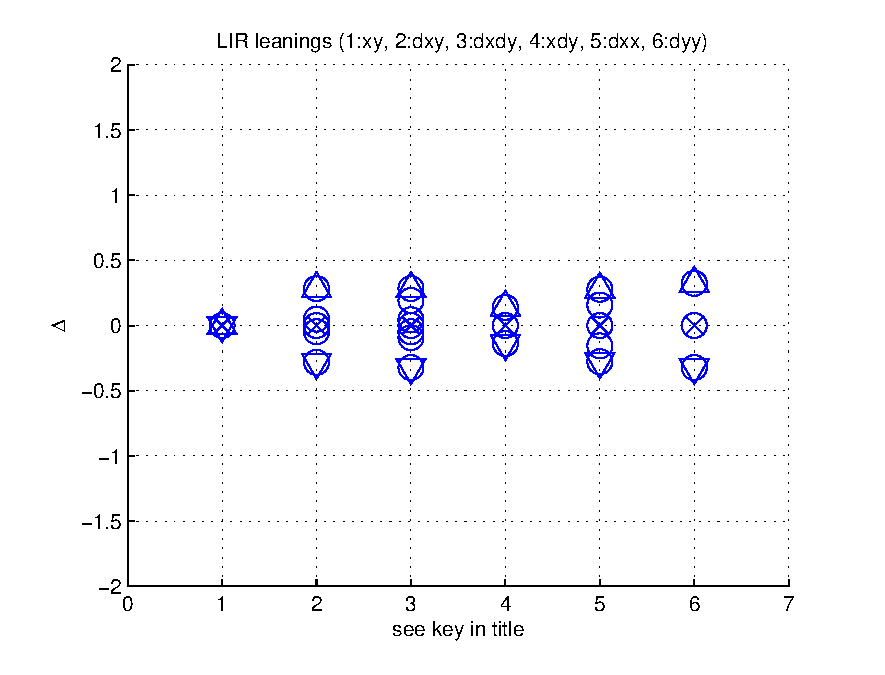
\includegraphics[scale=0.55]{LIRimgwTS000.eps}
\end{figure}
\begin{verbatim}
[x,y] = wTS(20,0.5,[1 5 15],[2 2 2]);
\end{verbatim}
\begin{figure}[!H]
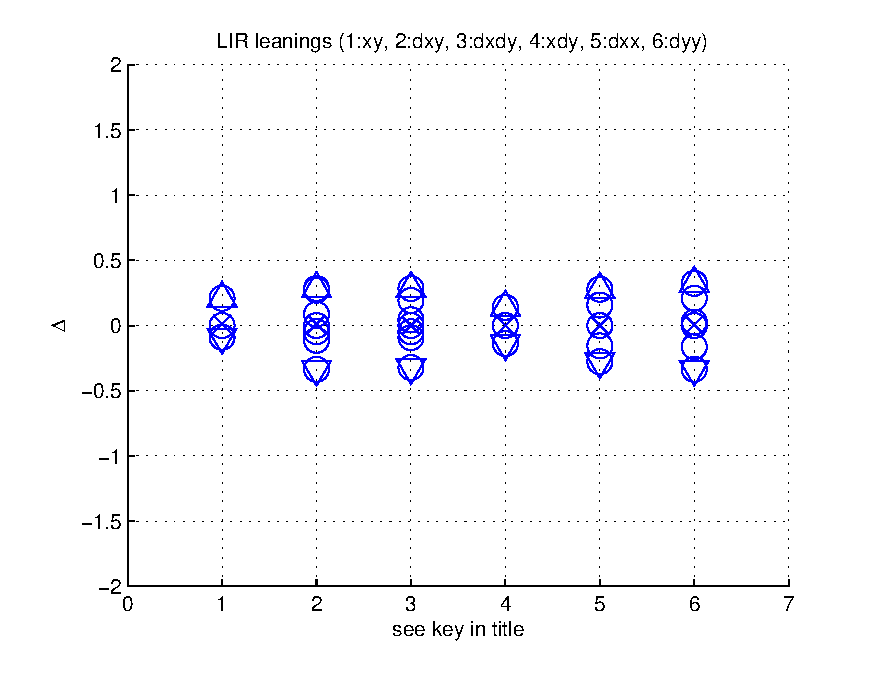
\includegraphics[scale=0.55]{LIRimgwTS050.eps}
\end{figure}

\end{document}



